\documentclass[a4paper, oneside]{book}
\usepackage[margin=2.5cm, bindingoffset=1cm]{geometry}
\linespread{1.5}
\usepackage{float}
\usepackage{csquotes}
\usepackage{subfig}
\usepackage{graphicx}
\usepackage{indentfirst}
\usepackage{fancyhdr}
\usepackage{array}
\usepackage[hidelinks]{hyperref}
\setlength{\parindent}{1cm}
\usepackage{tcolorbox}
\usepackage{multicol}
\usepackage{lmodern}
\usepackage{amsmath, amssymb}
\usepackage{listings}
\usepackage{xcolor}
\usepackage{accsupp}
% For images
\usepackage[inkscapelatex=false]{svg}
\usepackage{fontawesome5}
% For WP3 chart
\usepackage{pgfplots}
\pgfplotsset{compat=1.18}
\usepgfplotslibrary{polar}
\usepackage{lscape}
\usepackage{booktabs}

\pagestyle{fancy}
\renewcommand{\chaptermark}[1]{\markboth{\thechapter.\ \uppercase{#1}}{}}
\fancyhf{}
\fancyhead[C]{\textbf{\leftmark}}
\fancyfoot[C]{\thepage}
\renewcommand{\headrulewidth}{1pt}
\renewcommand{\footrulewidth}{1pt}
\usepackage[Conny]{fncychap}

\definecolor{codegreen}{rgb}{0,0.6,0}
\definecolor{codegray}{rgb}{0.5,0.5,0.5}
\definecolor{codepurple}{rgb}{0.58,0,0.82}
\definecolor{backcolour}{rgb}{0.95,0.95,0.92}

\lstdefinestyle{mystyle}{
    backgroundcolor=\color{backcolour},
    commentstyle=\color{codegreen},
    keywordstyle=\color{magenta},
    numberstyle=\tiny\color{codegray},
    stringstyle=\color{codepurple},
    basicstyle=\ttfamily\footnotesize,
    breakatwhitespace=false,
    columns=fullflexible,
    breaklines=true,
    postbreak=\raisebox{0ex}[0ex][0ex]{\ensuremath{\color{gray}\hookrightarrow\space}},
    captionpos=b,
    keepspaces=true,
    numbers=left,
    numbersep=5pt,
    showspaces=false,
    showstringspaces=false,
    showtabs=false,
    tabsize=4
}

\lstset{style=mystyle}

\title{AI4cybersecurity Project}
\author{reverseEkans}
\date{May 2025}

\renewcommand{\contentsname}{\bf Indice}
\renewcommand{\chaptername}{Capitolo}
  
\begin{document}
    %Frontespizio
    \begin{titlepage}
        \begin{center}
            \LARGE{\uppercase{Università degli Studi di Salerno}}\\
            \vspace{5mm}
            %Dipartimento
        	\uppercase{\normalsize \textbf{Dipartimento di Ingegneria dell'Informazione ed Elettrica e Matematica Applicata} }\\
        \end{center}
        
        \begin{figure}[H]
            \centering
            
\includegraphics[width=0.35\textwidth]{images/logo_unisa.png}
        \end{figure}
        
        \begin{center}
            % Corso di Laurea
        	\normalsize{ Corso di Laurea Magistrale in Ingegneria Informatica }\\
        	\vspace{15mm}
        	% Titolo
            {\Large{\bf \textbf{Security assessment of a
face recognition system}}}\\
        	\vspace{15mm}
            % Sottotitolo
            {\Large{reverseEkans - gruppo 10}}
            \vspace{10mm}
        \end{center}

        \begin{center}
            \begin{tabular}{ | c | c | c | c |} \hline
                \textbf{Nome} & \textbf{Cognome} & \textbf{Matricola} & \textbf{E-Mail} \\
                \hline
                Giuseppe Alfonso & Mangiola & 0622702372 & g.mangiola1@studenti.unisa.it \\
                \hline
                Emanuele & Relmi & 0622702368 & e.relmi@studenti.unisa.it\\
                \hline
                Francesco & Quagliuolo & 0622702412 & f.quagliuolo@studenti.unisa.it\\
                \hline
                Luca & Concilio & 0622702415 & l.concilio9@studenti.unisa.it\\
                \hline
            \end{tabular}
        \end{center}
        
        \vspace{20mm}
        
        %Anno Accademico
        \centering{\large \uppercase{Anno Accademico 2024/2025}}
    
    \end{titlepage}

    %Corpo del Documento
    \tableofcontents
    \clearpage
    \sloppy
    \hyphenpenalty=10000
    \exhyphenpenalty=10000
    
    \chapter*{Introduzione}
\markboth{INTRODUZIONE}{}
    Negli ultimi anni, l’Intelligenza Artificiale ha visto una crescita esponenziale in termini di popolarità, affidabilità e accessibilità economica, entrando a far parte della vita quotidiana in moltissimi settori. Le applicazioni basate su reti neurali sono ormai diffuse, facili da usare e alla portata di tutti, anche senza competenze specifiche, trovando spazio persino in contesti ludici. Un impatto significativo sicuramente lo si è riscontrato nel campo della sicurezza, dove l'IA viene progressivamente impiegata in ambiti che fino a poco tempo fa erano considerati esclusiva dell’intervento umano, grazie alla sua capacità di garantire prestazioni affidabili e costanti.
    Applicazioni come il controllo accessi, l’autenticazione sui dispositivi mobili, la videosorveglianza e il monitoraggio in spazi pubblici fanno largo uso di tecnologie biometriche, quali il riconoscimento delle impronte digitali, dell’iride e della voce, ognuna con specifici vantaggi in termini di precisione e contesto d’uso. Nello specifico, sono i sistemi di riconoscimento facciale spesso preferiti per la natura non invasiva, trainati dall’evoluzione dei sistemi di visione artificiale e delle reti neurali profonde.
    Tuttavia, come qualsiasi tecnologia, anche l’applicazione dell’Intelligenza Artificiale in contesti di sicurezza non è esente da potenziali vulnerabilità, che possono essere sfruttate da attaccanti per costruire exploit mirati a compromettere l’affidabilità dei sistemi. Ad esempio, è stato dimostrato che molti modelli di deep learning, pur essendo altamente accurati su immagini ``pulite'', possono essere ingannati da input artificialmente modificati. Tali input sono noti come \textit{adversarial examples} e consistono in perturbazioni impercettibili all’occhio umano, ma capaci di alterare drasticamente l’output del classificatore.
    Nel dominio della face recognition, questo tipo di attacco può avere implicazioni molto gravi: ad esempio, un volto opportunamente modellato, potrebbe essere riconosciuto come appartenente ad una determinata persona (\textit{error-specific}) oppure potrebbe essere etichettato erroneamente come appartenente ad un'identità qualsiasi, diversa da quella reale (\textit{error-generic}), consentendo così l’accesso a risorse riservate o l’elusione dei controlli. L’esistenza di queste vulnerabilità mina la fiducia nell’adozione su larga scala di questi sistemi, specialmente in ambiti ad alta criticità come aeroporti, strutture militari, banche e ambienti IoT.

    \begin{figure}[H]
        \centering
        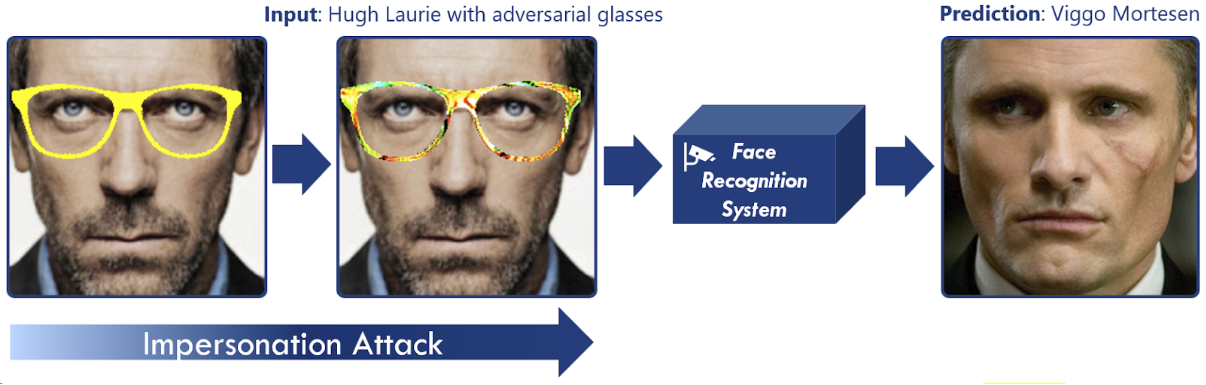
\includegraphics[width=0.95\textwidth]{images/impersonation_attack.png}
        \caption{Esempio di Face Recognition attack}
    \end{figure}

    \noindent Il presente progetto si propone di \textbf{valutare in modo sistematico la sicurezza di un sistema di face recognition} rispetto ad attacchi adversarial. A tal fine, ci siamo avvalsi di un sistema di riconoscimento facciale basato su un modello già esistente, del quale abbiamo preliminarmente valutato l’accuratezza su un test set appositamente costruito. Successivamente, il sistema è stato sottoposto a una serie di attacchi noti nella letteratura, sia di tipo error-generic che error-specific, al fine di analizzarne la risposta in presenza di input manipolati e valutarne l’eventuale degrado prestazionale, in particolare la difficoltà nel distinguere immagini autentiche da quelle contraffatte.
    Per approfondire il fenomeno della \textbf{trasferibilità} degli attacchi, gli stessi input avversari sono stati applicati anche a un secondo modello, basato su un’architettura differente, con l’obiettivo di indagare la capacità degli attacchi di conservare la propria efficacia anche su sistemi non direttamente conosciuti dall’attaccante, un aspetto cruciale nei contesti reali in cui spesso l’accesso al modello bersaglio non è esplicito.
    Infine, è stato implementato un meccanismo di difesa mirato a migliorare la robustezza del sistema originale nei confronti degli attacchi avversari, con l’intento di aumentarne l’affidabilità in scenari operativi.
    Il progetto si propone quindi come uno studio completo e sperimentale sulla robustezza dei moderni sistemi di face recognition, offrendo un contributo all’analisi delle loro vulnerabilità e alla progettazione di contromisure.
    Il lavoro è suddiviso nei seguenti capitoli:
        \begin{itemize}
            \item \textbf{Capitolo 1:} descrizione del dataset, criteri di selezione delle immagini, struttura del test set, pre-processing dei dati e analisi delle performance del modello;
            
            \item \textbf{Capitolo 2:} generazione di Adversarial Examples e analisi delle performance del modello;
            
            \item \textbf{Capitolo 3:} verifica della trasferibilità degli attacchi su un secondo modello;
            
            \item \textbf{Capitolo 4:} implementazione e valutazione di una strategia di difesa sul modello originale;
            
            \item \textbf{Capitolo 5:} conclusioni e riflessioni finali.
        \end{itemize}
    \chapter{Dataset e Setup Sperimentale}
    \section{Obiettivi della fase iniziale}
        Questa prima fase del progetto ha conseguito i seguenti obiettivi:
            \begin{enumerate}
                \item Costruire un test set realistico, bilanciato e rappresentativo per la valutazione delle performance facciali.
                \item Valutare le prestazioni del modello NN1 in condizioni non perturbate, per stabilire una baseline di riferimento.
                \item Definire un ambiente stabile e riproducibile per l’esecuzione controllata di attacchi adversarial e successive difese.
            \end{enumerate}

        \noindent I risultati ottenuti in questa fase costituiscono la base sperimentale su cui si innesteranno, nei capitoli successivi, l’analisi degli attacchi e l’efficacia delle contromisure proposte.

    \section{Ambiente di sviluppo}
        Tutte le sperimentazioni sono state condotte in ambiente separato \textit{conda} (\texttt{anaconda} o \texttt{miniconda}) utilizzando \texttt{Python 3.10}, sfruttando \textit{Jupyter Notebook}, \texttt{PyTorch} come framework di deep learning e \texttt{Adversarial Robustness Toolbox (ART)} per la generazione e gestione degli attacchi adversarial. I notebook sono stati sviluppati ed eseguiti su \textit{Visual Studio Code}, sfruttando una GPU.
        Di seguito si elencano le principali dipendenze utilizzate:
            \begin{itemize}
                \item \texttt{torch==2.x}, \texttt{torchvision}
                
                \item \texttt{numpy}, \texttt{matplotlib}
                
                \item \texttt{adversarial-robustness-toolbox}
                
                \item \texttt{facenet-pytorch}, \texttt{tensorflow}
            \end{itemize}

    \section{VGG-Face2 e costruzione del test set}
        Per valutare la robustezza del sistema di riconoscimento facciale, è stato utilizzato un modello (\texttt{InceptionResnetv1}) pre-addestrato sul dataset \texttt{VGG-Face2}, uno dei benchmark più noti in ambito face recognition. Questo dataset contiene oltre 3 milioni di immagini raccolte dal web e suddivise in più di 9.000 identità, con una forte variabilità in termini di età, etnia, pose e condizioni di illuminazione.
        Ai fini di questo progetto, come da requisiti, sono state selezionate manualmente \textbf{100 identità} dal training set del dataset, ciascuna rappresentata da almeno \textbf{20 immagini}, per un totale complessivo di \textbf{2408 immagini}.
        Per garantire variabilità intra-classe (espressioni, pose, sfondi) e inter-classe (etnie, sesso, età), le immagini sono state accuratamente filtrate. Durante una fase preliminare di cleaning sono stati rimossi file duplicati, volti oscurati o mal ritagliati.
        Tale test set è stato utilizzato sia per la valutazione iniziale delle performance, sia come base per generare gli \textit{adversarial samples}.
        Il test set è stato organizzato secondo la struttura prevista da \texttt{torchvision.datasets.ImageFolder}, con una directory principale e una sottocartella per ciascuna identità (es. \texttt{dataset/Test\_set/n000202/}, \texttt{dataset/Test\_set/n000201/}, \ldots), rendendo agevole il caricamento e l’etichettatura automatica.
            \begin{figure}[H]
                \centering
                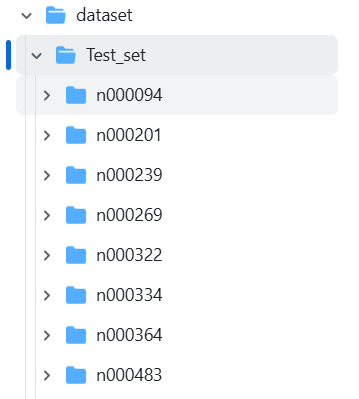
\includegraphics[width=0.55\textwidth]{images/Test_set.png}
                \caption{Test set organization}
            \end{figure}

        \noindent Durante la fase di importazione con \texttt{PyTorch}, per rendere le immagini conformi ai vincoli del modello riguardo gli input, sono state applicate una serie di trasformazioni:
            \begin{itemize}
                \item Resize a $160 \times 160$ pixel, come richiesto dal modello \texttt{InceptionResnetV1}, che accetta in input immagini quadrate di tale dimensione poichè risulta essere ottimizzato per questa risoluzione;
                \item Conversione in tensori;
                \item Normalizzazione con \texttt{mean} e \texttt{std} impostati a $[0.5, 0.5, 0.5]$
            \end{itemize}
            
        \noindent Il caricamento è stato gestito tramite un \texttt{DataLoader} con \texttt{batch\_size = 32} e \texttt{shuffle = False}, al fine di mantenere fisso l’ordine delle immagini per il confronto tra predizioni clean e adversarial. \\            
        
        \noindent \textbf{Distribuzione del test set:}
            \begin{itemize}
                \item Numero totale identità: 100
                \item Numero medio di immagini per identità: 24.08
                \item Dimensione media immagine: $160 \times 160 \times 3$
            \end{itemize}

    \section{Modello NN1}
        Il modello di partenza (denominato \textbf{NN1}) è una rete neurale convoluzionale profonda, basata sull’architettura \texttt{InceptionResnetV1}. Questo modello è stato pre-addestrato sul dataset \texttt{VGG-Face2} ed è reso disponibile tramite la libreria \texttt{facenet-pytorch}. È progettato per il riconoscimento facciale e restituisce, per ogni immagine in input, un vettore di \textbf{512 caratteristiche} (embedding) che rappresentano la firma numerica del volto nel dominio euclideo.
        A differenza dell’uso canonico in FaceNet (dove si confrontano direttamente gli embedding tra volti), in questo progetto il modello è stato utilizzato in modalità \verb|classify=True|, che abilita un layer di classificazione finale su 8.631 identità del dataset \texttt{VGG-Face2}. Le etichette corrispondenti ai samples presenti nel dataset sono state ottenuto caricando il file di riferimento \texttt{rcmalli\_vggface\_labels\_v2.npy}, reso disponibile dall'omonima repository Github. Infine, il modello così ottenuto è stato spostato, se disponibile, sulla GPU, per ridurre i tempi di calcolo.
        A partire dalla struttura del test set, le immagini sono state caricate e preprocessate tramite le trasformazioni descritte in precedenza. Ogni immagine è stata associata alla rispettiva etichetta di classe, secondo l’organizzazione delle sottocartelle prevista da ImageFolder. Per ottimizzare i tempi di esecuzione nelle iterazioni successive, i tensori contenenti immagini (\texttt{x\_test}) e label (\texttt{y\_test}) sono stati salvati in un file \texttt{.pt}, evitando così la necessità di ricostruire il dataset a ogni avvio.
        Durante la valutazione, il modello è stato utilizzato in modalità \texttt{eval()}, senza aggiornamento dei pesi, al fine di valutarne la robustezza così com'è, senza alcun fine-tuning. La fase di testing della rete originale ha previsto l’iterazione sull’intero test set, durante la quale ciascuna immagine è stata elaborata dal modello per produrre una predizione. Per ogni immagine, è stata selezionata la classe corrispondente alla probabilità massima in output, mentre la classe reale è stata recuperata dal test set di riferimento. La predizione è stata poi confrontata con la label reale per verificarne la correttezza.
        L’intero processo è stato eseguito all’interno di un blocco \texttt{torch.no\_grad()}, che disattiva il calcolo del gradiente durante l’inferenza, riducendo il consumo di memoria e velocizzando l’esecuzione. Al termine, l’accuratezza è stata calcolata come rapporto tra il numero di predizioni corrette e il numero totale di immagini nel test set, restituendo così il valore percentuale finale di accuratezza del classificatore.
        Nello specifico, l’accuratezza ottenuta sul test set “clean” (non perturbato) è stata pari al \textbf{92{,}32\%}, con \textbf{2.223} predizioni corrette su un totale di \textbf{2.408} immagini.
        Questa configurazione ha permesso di utilizzare NN1 come solido punto di riferimento per confrontare l’impatto degli attacchi avversari nei capitoli successivi.
    \chapter{Adversarial Attacks}
    \section{Contesto teorico}
        Nonostante le reti neurali profonde abbiano raggiunto prestazioni straordinarie in molteplici task visivi, tra cui il riconoscimento facciale, la continua ricerca di tecniche in grado di manipolare l'esito del riconoscimento, le rende potenzialmente vulnerabili ad attacchi di tipo adversarial.
        Gli \textit{adversarial examples} sono immagini appositamente modificate tramite perturbazioni minime e impercettibili per l’occhio umano, in grado di causare un’errata classificazione da parte del modello. Queste perturbazioni sono costruite sfruttando la sensibilità del modello ai gradienti: piccoli cambiamenti nella direzione di maggiore variazione dell’output (calcolati tramite il gradiente della funzione di loss rispetto all’input) possono spostare l’immagine nello spazio delle feature, portando il modello a cambiare la propria predizione anche se, visivamente, l’immagine resta praticamente identica. 
        Questo fenomeno, apparentemente paradossale, è particolarmente preoccupante nell'ambito della cybersecurity, dove il riconoscimento facciale viene utilizzato in sistemi di controllo accessi, autenticazione biometrica, videosorveglianza e verifica dell' identità.
        Esistono due principali categorie di attacco:
            \begin{itemize}
                \item \textbf{Error-generic}: l'obiettivo è far sì che un'immagine venga classificata in una qualsiasi classe diversa da quella corretta.
                
                \item \textbf{Error-specific}: l'obiettivo è far classificare l'immagine in una classe specifica a scelta dell'attaccante.
            \end{itemize}

        \noindent In ambito reale, un attacco error-generic potrebbe portare al rifiuto di accesso per un utente legittimo, mentre un attacco error-specific potrebbe essere usato da un attaccante per impersonare un’altra persona.
        Nel nostro progetto, abbiamo valutato la \textbf{robustezza del modello NN1} attraverso cinque diversi attacchi \textbf{non mirati} (\textit{untargeted}), ovvero attacchi che si limitano a forzare un errore di classificazione, senza specificare la classe obiettivo, e analogamente gli stessi, eccezion fatta per DeepFool, applicati con lo scopo di una misclassificazione verso una specifica classe, quindi \textbf{mirati} (\textit{targeted}).

    \section{Approccio sperimentale}
        Tutti gli attacchi sono stati implementati tramite la libreria \texttt{Adversarial Robustness Toolbox (ART)}. I test sono stati condotti su tutto il test set e per ciascun attacco è stata calcolata la variazione dell’Accuracy top-1 del modello NN1 in funzione del parametro $\epsilon$.
        \textbf{Nota:} Sebbene la traccia del progetto raccomandasse di fermarsi a $\epsilon = 0.05$, abbiamo esteso la sperimentazione includendo i valori:
        
        \[
        \epsilon \in \{0.001,\ 0.005,\ 0.01,\ 0.025,\ 0.05,\ 0.075,\ 0.1\}
        \]
        
        \noindent Questa scelta ha permesso di osservare il comportamento del modello anche oltre i limiti raccomandati, per analizzarne la resistenza in scenari estremi.

    \section{Non-Targeted Adversarial Attacks}
        Gli attacchi non-targeted hanno l'obiettivo di indurre un errore nel classificatore senza forzare la predizione verso una classe specifica, valutandone l'impatto sul classificatore NN1 tramite metriche quantitative e curve di valutazione della sicurezza (\textbf{security evaluation curves}).

        \subsection{Fast Gradient Sign Method (FGSM)}
            Il Fast Gradient Sign Method (FGSM) è un attacco one-shot basato sul gradiente  della funzione di perdita della rete rispetto all'immagine di input. Esso applica una  perturbazione $\epsilon$ proporzionale al segno del gradiente, per allontanarsi dalla classe vera di un $\epsilon$, come mostrato nella seguente formula:
                $$
                x_{\text{adv}} = x + \epsilon \cdot \text{sign}(\nabla_x \mathcal{L}(h(x, w), y))
                $$

            \noindent Nel nostro esperimento, l'attacco è stato eseguito iterando su diversi valori di $\epsilon$:
                $$
                \epsilon \in \{0.001, 0.005, 0.01, 0.025, 0.05, 0.075, 0.1\}
                $$

            \noindent con l'obiettivo di causare una classificazione errata mantenendo una perturbazione impercettibile all'occhio umano, gli adversarial examples sono stati generati a partire dai campioni del test set mediante il FGSM, utilizzando l’implementazione fornita dalla libreria ART. Per ottimizzare l’efficienza computazionale, gli esempi avversari sono stati elaborati in batch di dimensione 64 e successivamente sottoposti al modello NN1 per la fase di inferenza.
            Il processo di valutazione dell’accuratezza segue lo stesso schema già descritto nella sezione precedente, con l’aggiunta di operazioni di normalizzazione e conversione tra tensori e array, necessarie per garantire la compatibilità tra ART e PyTorch.
            Per evitare la rigenerazione degli esempi ad ogni esecuzione, ciascun set avversario è stato salvato su file, con riferimento esplicito al valore di $\epsilon$ utilizzato.
            Infine, il grafico della Security Evaluation Curve mostra l’andamento dell’accuratezza del modello al crescere dell’intensità dell’attacco, evidenziando la relazione inversa tra la robustezza del classificatore e l’entità della perturbazione introdotta.

            \subsubsection*{Risultati sperimentali}
                \noindent L'attacco è stato testato su un range di valori di $\epsilon$. I risultati mostrano un'attesa degradazione delle prestazioni del classificatore NN1 all'aumentare della perturbazione. A partire da $\epsilon$ contenuti il sistema si è dimostrato resiliente agli attacchi, mentre spostandosi ad ordini di grandezza superiori, il modello mostra una vulnerabilità visibile.

                    \begin{itemize}
                        \item $\epsilon = 0.001$: accuratezza 91.28\%, perturbazione media 0.0009
                        
                        \item $\epsilon = 0.010$: accuratezza 44.44\%, perturbazione media 0.0094
                        
                        \item $\epsilon = 0.025$: accuratezza 9.05\%, perturbazione media 0.0235
                        
                        \item $\epsilon = 0.100$: accuratezza 0.46\%, perturbazione media 0.0924
                    \end{itemize}

                \noindent La Security Evaluation Curve mostrata in figura fornisce una rappresentazione visiva chiara dell’impatto degli attacchi FGSM sul modello NN1. La curva mette in evidenza la decrescita in accuratezza del classificatore all’aumentare dell’intensità della perturbazione avversaria.
                In particolare, si osserva una riduzione di oltre il 50\% dell’accuratezza originale per una perturbazione pari a circa 0.01, mentre in corrispondenza del valore massimo consentito ($\epsilon$ = 0.05) mostra un’accuratezza praticamente nulla.

                    \begin{figure}[H]
                        \centering
                        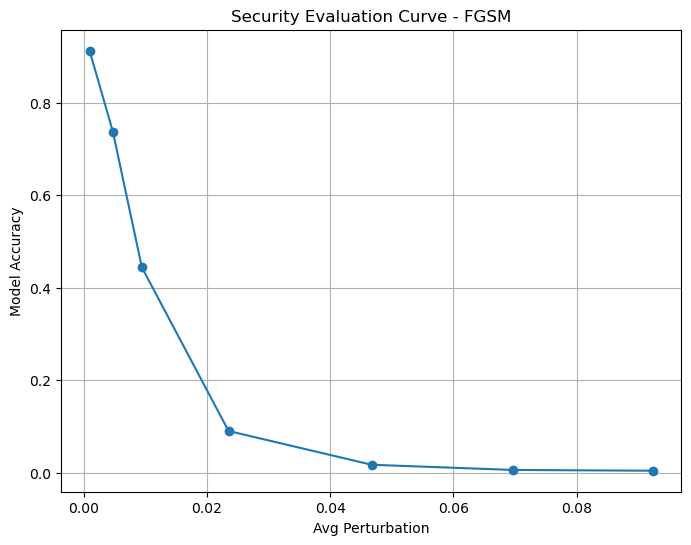
\includegraphics[width=0.65\textwidth]{images/evaluation_curve_fgsm.png}
                        \caption{Security Evaluation Curve per l'attacco FGSM (non-targeted)}
                    \end{figure}

        \subsection{Basic Iterative Method (BIM)}
            Il Basic Iterative Method (BIM) è un'estensione dell'attacco FGSM in cui la perturbazione viene applicata in modo iterativo, con piccoli step e clipping finale per mantenere l'intensità sotto controllo. \\
            La formula iterativa dell’attacco è:
                \[
                x_t' = x_{t-1} + \alpha \cdot \text{sign} \left( \nabla_x \mathcal{L}(h(x_{t-1}, w), y) \right)
                \]

            \noindent dove $\alpha$ è la quantità di rumore aggiunta ad ogni iterazione e $\boldsymbol{t}$  rappresenta il numero di iterazioni. L'idea di aggiungere piccole quantità di rumore in diversi step multipli aumenta le probabilità di misclassificare un'immagine rispetto all'attacco originale.

            \subsubsection*{Risultati sperimentali}
                \noindent Per l'attacco Basic Iterative Method (BIM) sono stati eseguiti esperimenti variando sia il parametro $\epsilon$ sia il numero massimo di iterazioni $t \in \{5, 10, 20\}$. I risultati, in linea con quanto introdotto, evidenziano un chiaro incremento dell'efficacia dell'attacco all'aumentare di entrambi i parametri.
                
                \begin{itemize}
                    \item Per $\epsilon = 0.001$ l’accuratezza rimane invariata intorno al 91.3\%, indipendentemente dal numero di iterazioni.
                    
                    \item Per $\epsilon = 0.01$, l’accuratezza cala drasticamente fino al 20.60\% con $t=20$.
                    
                    \item Per $\epsilon \geq 0.025$, l’accuratezza scende sotto l’1\% già a 5 iterazioni, fino ad azzerarsi con $t \geq 10$.
                \end{itemize}
                
                \noindent L’aumento del numero di iterazioni risulta particolarmente efficace nel regime di $\epsilon$ intermedio (es. 0.01–0.05), mentre a valori molto elevati l’accuratezza crolla anche con pochi passi. La curva mostra come l’attacco riesca a compromettere il modello con perturbazioni limitate ma iterative.

                \begin{figure}[H]
                    \centering
                    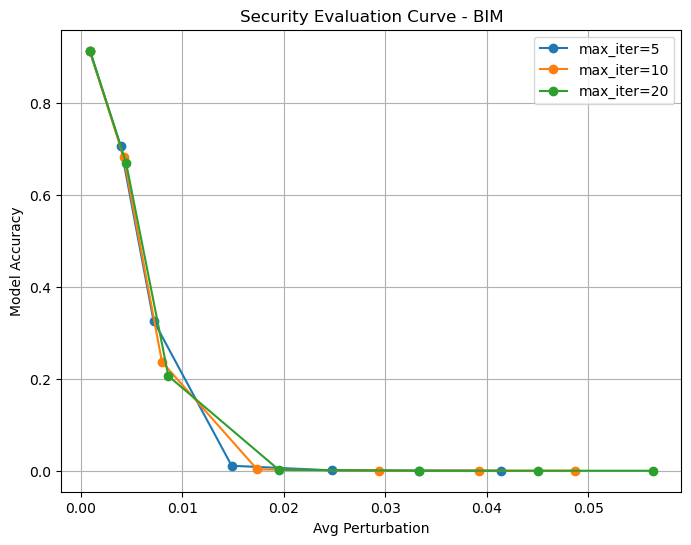
\includegraphics[width=0.75\textwidth]{images/evaluation_curve_bim.png}
                    \caption{Security Evaluation Curve per l'attacco BIM (non-targeted)}
                \end{figure}

                \noindent Analizzando la curva, si osserva che, a parità di accuratezza del modello, un numero maggiore di iterazioni consente di ingannare il classificatore con perturbazioni di intensità inferiore. In particolare, le curve corrispondenti a 10 e 20 iterazioni raggiungono un’accuratezza prossima allo 0\% più rapidamente rispetto a quella relativa a 5 iterazioni, evidenziando una maggiore efficacia dell’attacco al crescere del numero di passi di ottimizzazione.

        \subsection{Projected Gradient Descent (PGD)}
            Il Projected Gradient Descent (PGD) rappresenta una generalizzazione iterativa dell’attacco FGSM. Alla base di PGD c’è l’idea di eseguire piccoli passi iterativi seguendo il gradiente della funzione di perdita rispetto all'input, aggiornando progressivamente l'immagine avversaria. Dopo ogni passo, l’immagine perturbata viene proiettata nuovamente all’interno della sfera di raggio $\epsilon$ centrata sull’immagine originale ($\epsilon$ ball).
            La formula iterativa è simile a quella di BIM, ma include la funzione di proiezione $\pi$ a ogni passo:
            
            \[
            x_t' = \Pi_\epsilon \left( x_{t-1} + \alpha \cdot \text{sign} \left( \nabla_x \mathcal{L}(h(x_{t-1}, w), y) \right) \right)
            \]
            
            \noindent dove $\Pi$ è la funzione di proiezione nella sfera L$_\infty$, $\alpha$ è il passo, e $\mathcal{L}$ la loss.

            \subsubsection*{Risultati sperimentali}
                \noindent L'attacco Projected Gradient Descent (PGD), noto per essere una versione iterativa più robusta del FGSM e di BIM, è stato testato con due valori di iterazioni massime $t \in \{10, 20\}$ e diversi valori di $\epsilon$.
                
                \begin{itemize}
                    \item Per valori molto bassi di $\epsilon$ (0.001), il modello mantiene un’alta accuratezza (91.3\%), anche dopo 20 iterazioni.
                    \item A partire da $\epsilon = 0.01$, l’accuratezza crolla drasticamente, si scende al 25.5\% con $t=10$ e al 20.9\% con $t=20$.
                    \item Per $\epsilon \geq 0.025$, il modello viene completamente compromesso: l’accuratezza si avvicina allo 0\%, anche con perturbazioni medie contenute.
                \end{itemize}
                
                \noindent I risultati dimostrano l’efficacia dell’attacco PGD, in grado di abbattere rapidamente l’accuratezza del classificatore anche con perturbazioni visivamente impercettibili. L’aumento di iterazioni da 10 a 20 migliora leggermente l’efficacia dell’attacco nei range intermedi di $\epsilon$.

                \begin{figure}[H]
                    \centering
                    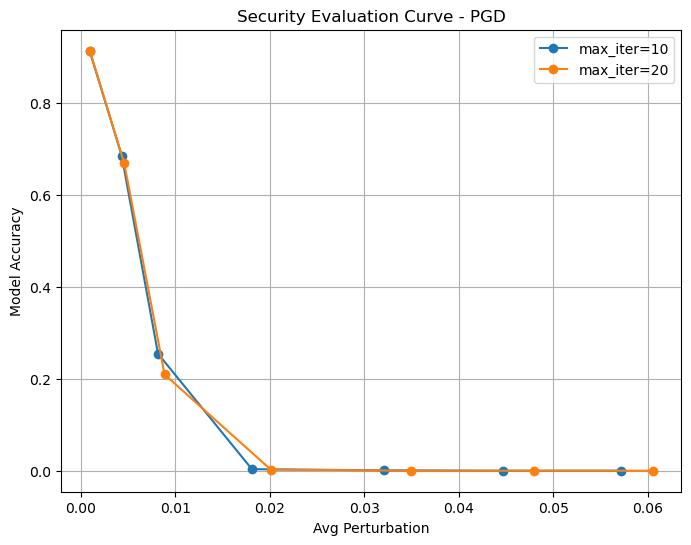
\includegraphics[width=0.75\textwidth]{images/evaluation_curve_pgd.png}
                    \caption{Security Evaluation Curve per l'attacco PGD (non-targeted)}
                \end{figure}

        \subsection{DeepFool}
            L’attacco \textbf{DeepFool} è una tecnica iterativa per la generazione di perturbazioni minime che portino un classificatore lineare, o non, a misclassificare l'output. A differenza degli attacchi gradient-based più aggressivi, come PGD, DeepFool mira specificamente a trovare la perturbazione minima necessaria a spingere l'immagine oltre il confine decisionale del classificatore, rappresentato da un iperpiano, garantendo quindi un attacco più ``preciso'' in termini di ottimizzazione dell'energia della perturbazione. \\
            La formula alla base dell’attacco (nella versione binaria) si ispira a:
                \[
                r^* = - \frac{f(x)}{\| \nabla f(x) \|^2} \cdot \nabla f(x)
                \]
            
            \subsubsection*{Risultati sperimentali}
                \noindent Nel nostro esperimento, abbiamo selezionato \textbf{50 immagini casuali} dal test set, impostando come parametri principali un \textit{overshoot} $\epsilon = 0.02$ e massimo \textit{numero di iterazioni} pari a 5, con i primi 10 gradienti dominanti (classi più probabili) considerati.
                L’accuratezza residua del modello dopo l’attacco è risultata pari a \textbf{84.00\%}, con una \textbf{fooling rate} complessiva del \textbf{16.00\%}. Il valore medio di perturbazione $L\infty$ applicato è stato molto contenuto: \textbf{0.00163}, a conferma della natura parsimoniosa dell’attacco.
                
                \begin{figure}[H]
                    \centering
                    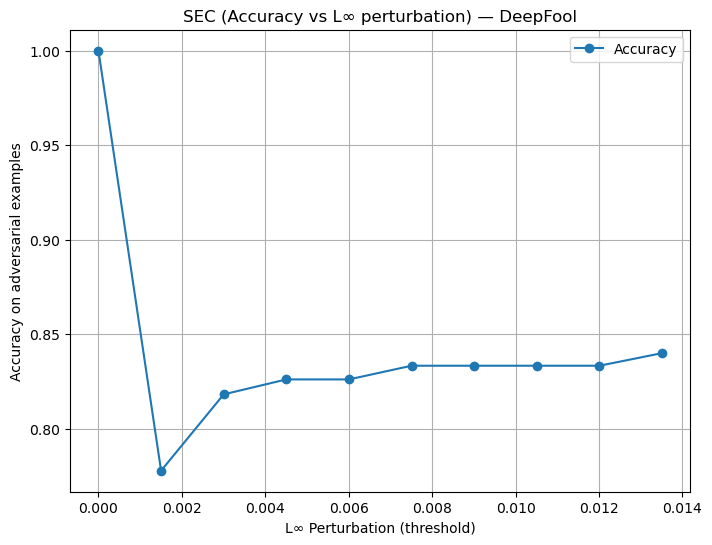
\includegraphics[width=0.6\linewidth]{images/evaluation_curve_deepfool.png}
                    \caption{Security Evaluation Curve (SEC) --- Accuratezza vs. soglia $L\infty$ (DeepFool)}
                \end{figure}
                
                \noindent Nel primo grafico è riportata la \textbf{Security Evaluation Curve (SEC)}, che mostra l’andamento dell’accuratezza del classificatore al variare del valore soglia massimo di perturbazione $L\infty$. Si osserva una prima brusca caduta dell’accuratezza anche per soglie molto piccole, seguita da una stabilizzazione intorno all’83–84\%: questo suggerisce che una porzione delle immagini avversarie riesce ad alterare la previsione già con minime modifiche.
                
                \begin{figure}[H]
                    \centering
                    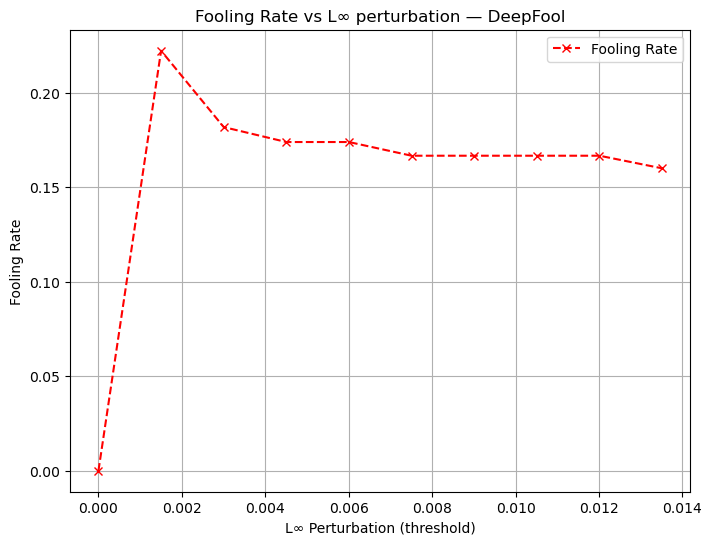
\includegraphics[width=0.6\linewidth]{images/fooling_rate_deepfool.png}
                    \caption{Tasso di inganno (Fooling Rate) vs. soglia $L\infty$ (DeepFool)}
                \end{figure}
                
                \noindent Il secondo grafico mostra la \textbf{fooling rate}, ovvero la percentuale di immagini la cui predizione è stata alterata, rispetto alla soglia massima di perturbazione. Si nota un picco iniziale (oltre il 20\%) per soglie minime, seguito da una graduale decrescita. Questo comportamento è coerente con quanto evidenziato in letteratura, dove viene mostrato come le perturbazioni ottimali di DeepFool tendano a concentrarsi su un sottile margine decisorio, risultando estremamente efficaci anche a bassissime magnitudini. Tuttavia, al crescere della soglia, il numero di immagini ``foolabili'' non aumenta proporzionalmente: ciò indica una certa robustezza intrinseca per una porzione del dataset, o l’inadeguatezza del metodo DeepFool su immagini più complesse (in quanto è un attacco non-targeted e localmente lineare).
                Questo andamento è dunque assolutamente plausibile e rafforza il ruolo di DeepFool come attacco utile per valutare con maggior precisione la vulnerabilità del modello, senza ricorrere a grandi perturbazioni.
            
        \subsection{Carlini-Wagner (CW) $L\infty$}
            \noindent L’attacco Carlini-Wagner (CW) è tra i più noti ed efficaci attacchi basati sul gradiente. Si fonda sulla formulazione di un problema di ottimizzazione vincolata, in cui l’obiettivo è minimizzare l’intensità della perturbazione necessaria a causare una classificazione errata.
            Rispetto ad altri metodi, come DeepFool, l’attacco CW risulta computazionalmente più oneroso, in quanto ad ogni iterazione l’algoritmo esplora diverse regioni di decisione proiettando la perturbazione in ciascuna di esse, confrontandone la distanza dal campione originale per selezionare quella che minimizza la norma del rumore aggiunto.
            Nel caso della norma $L\infty$, il problema si può riassumere come:
            \[
            \min \| \delta \|_\infty \quad \text{such that} \quad f(x + \delta) \ne y
            \]
            
            \noindent In questa sezione valutiamo l'efficacia dell'attacco non-targeted, variando l'apprendimento ($\text{learning\_rate} \in \{0.01, 0.1\}$), la costante iniziale ($\text{init\_const} \in \{0.01, 0.1\}$) e il numero massimo di iterazioni ($\text{max\_iter} \in \{1, 10, 20\}$). I risultati si riferiscono ad un sottoinsieme casuale di 20 immagini selezionate dal test set.
            
            \begin{figure}[H]
                \centering
                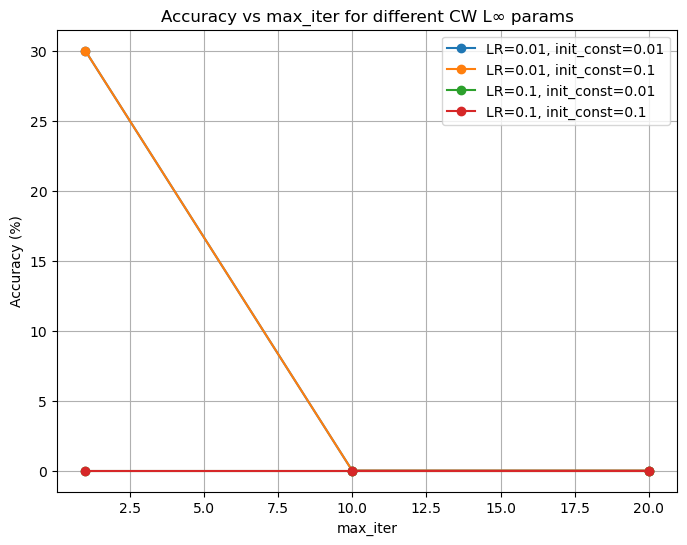
\includegraphics[width=0.65\textwidth]{images/cw_non_targeted_accuracy.png}
                \caption{Accuracy vs \texttt{max\_iter} per diversi parametri dell'attacco CW $L\infty$ (non-targeted).}
                \label{fig:cw-nt-accuracy}
            \end{figure}
            
            \noindent Come visibile in Figura~\ref{fig:cw-nt-accuracy}, l'attacco si dimostra estremamente efficace. Per $\text{learning\_rate} = 0.1$ l’accuratezza del modello scende immediatamente a $0\%$ indipendentemente da $\text{max\_iter}$ e $\text{init\_const}$, mentre con $\text{learning\_rate} = 0.01$ e $\text{max\_iter} = 1$ l’attacco è meno potente, riuscendo a mantenere un’accuratezza residua del $30\%$. Già a $\text{max\_iter} = 10$ l’attacco diventa efficace anche in questo scenario, abbattendo completamente le prestazioni del classificatore.
            
            \begin{figure}[H]
                \centering
                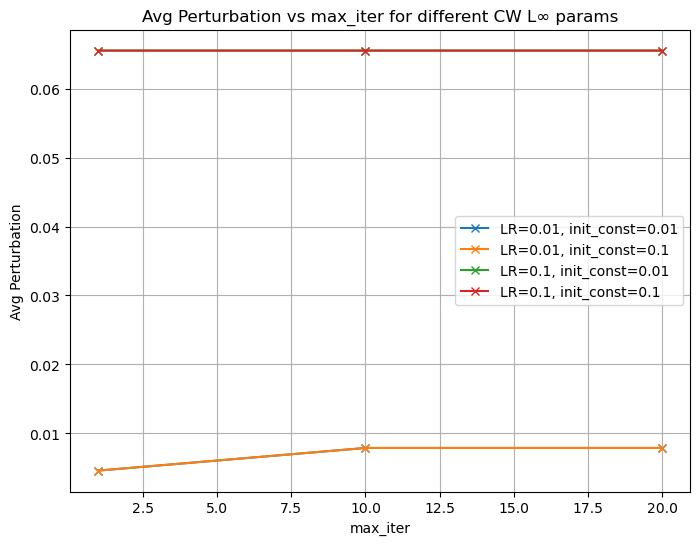
\includegraphics[width=0.65\textwidth]{images/cw_non_targeted_perturbation.png}
                \caption{Avg perturbation vs \texttt{max\_iter} per diversi parametri dell'attacco CW $L\infty$ (non-targeted).}
                \label{fig:cw-nt-perturbation}
            \end{figure}
            
            \noindent La figura~\ref{fig:cw-nt-perturbation} mostra come le perturbazioni siano controllate e in generale molto limitate, soprattutto per $\text{learning\_rate} = 0.01$, dove si rimane sotto lo 0.01 anche a 20 iterazioni. Al contrario, l’uso di un tasso di apprendimento più elevato porta a perturbazioni stabili ma più marcate ($\sim 0.065$), comunque sufficienti per ingannare completamente il modello.
            
            \begin{figure}[H]
                \centering
                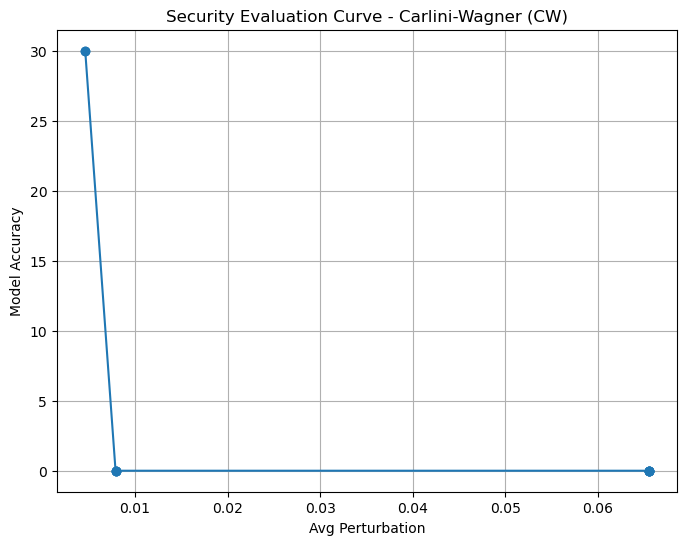
\includegraphics[width=0.65\textwidth]{images/cw_unt_ec.png}
                \caption{Security Evaluation Curve per CW $L\infty$ (non-targeted): accuratezza vs perturbazione media.}
                \label{fig:cw-nt-sec}
            \end{figure}
            
            \noindent La \textbf{Security Evaluation Curve} (Figura~\ref{fig:cw-nt-sec}) evidenzia la forte correlazione inversa tra perturbazione e accuratezza. L’attacco si conferma altamente efficace anche con perturbazioni estremamente contenute: l’unico punto con accuracy significativamente diversa da zero ($30\%$) corrisponde a $\epsilon \approx 0.0046$. Per perturbazioni superiori, l’attacco riesce sistematicamente a compromettere la classificazione.

        \subsection{Carlini-Wagner (CW) $L2$}
            In questo esperimento abbiamo applicato l'attacco Carlini-Wagner nella variante $L2$ e in modalità non-targeted direttamente alla rete NN1. Sono state esplorate diverse configurazioni dei parametri: \texttt{learning\_rate} $\in \{0.01, 0.1\}$, \texttt{initial\_const} $\in \{0.01, 0.1\}$ e \texttt{max\_iter} $\in \{1, 10, 20\}$. I risultati ottenuti sono rappresentati nei grafici in Figura~\ref{fig:cw_untarg_l2_acc}, \ref{fig:cw_untarg_l2_pert} e \ref{fig:cw_untarg_l2_sec}.
            
            \begin{figure}[H]
                \centering
                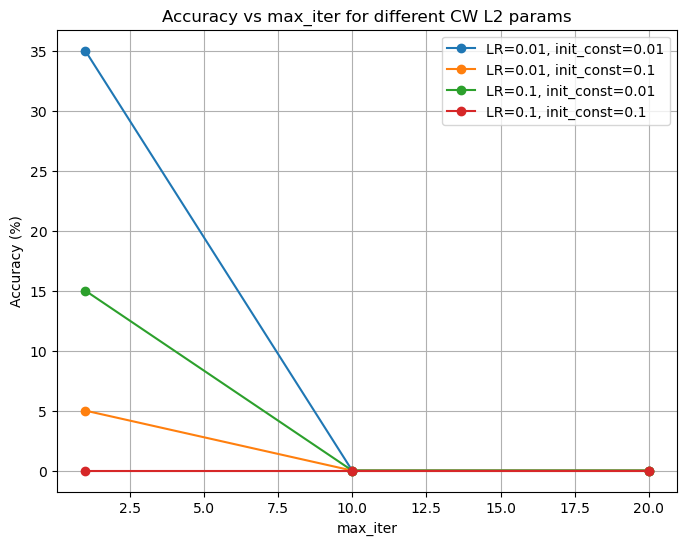
\includegraphics[width=0.6\textwidth]{images/accvsmaxl2.png}
                \caption{Accuracy vs max\_iter per Carlini \& Wagner $L^2$ (Non-targeted, NN1)}
                \label{fig:cw_untarg_l2_acc}
            \end{figure}
            
            \begin{figure}[H]
                \centering
                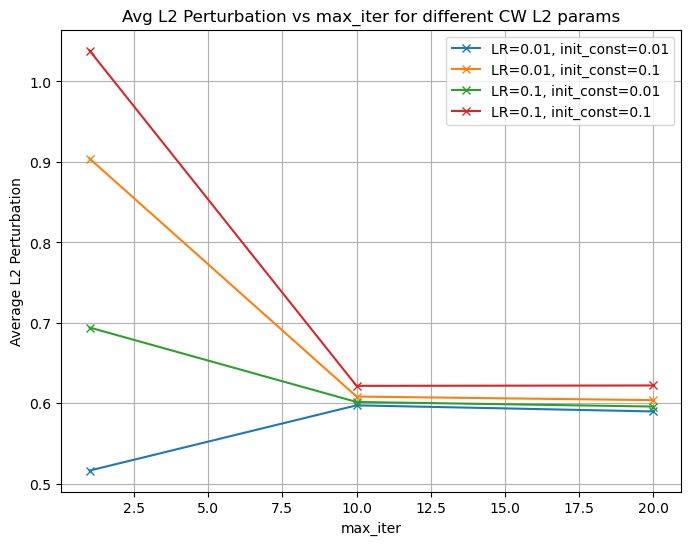
\includegraphics[width=0.6\textwidth]{images/avgpub_vs_maxiter_l2.png}
                \caption{Avg $L^2$ Perturbation vs max\_iter per Carlini \& Wagner $L^2$ (Non-targeted, NN1)}
                \label{fig:cw_untarg_l2_pert}
            \end{figure}
            
            \begin{figure}[H]
                \centering
                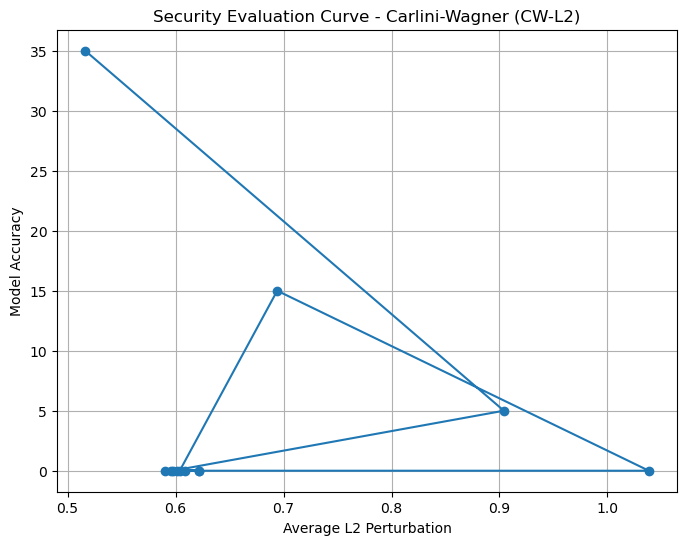
\includegraphics[width=0.6\textwidth]{images/sec_unt_cw_l2.png}
                \caption{Security Evaluation Curve per Carlini \& Wagner $L^2$ (Non-targeted, NN1)}
                \label{fig:cw_untarg_l2_sec}
            \end{figure}
            
            \subsection{Risultati sperimentali}
                L'attacco Carlini-Wagner $L2$ in modalità non-targeted si è dimostrato altamente efficace nel compromettere le predizioni della rete NN1. Per configurazioni con \texttt{max\_iter} elevate, l’accuratezza residua del modello si riduce rapidamente fino allo $0\%$, evidenziando che la rete è completamente ingannata dai campioni avversari generati.
                Nelle configurazioni con \texttt{max\_iter=1}, l’attacco non raggiunge lo stesso livello di successo, ma riesce comunque ad abbattere l'accuratezza fino al $5\%$–$35\%$, in funzione del valore di \texttt{init\_const} e \texttt{learning\_rate}. Al crescere delle iterazioni, l’attacco converge verso perturbazioni più “efficaci” e meno intense, con valori medi di norma $L2$ compresi tra $0.59$ e $0.62$.
                La \textit{security evaluation curve} evidenzia una forte correlazione inversa tra la norma della perturbazione e l’accuratezza del classificatore: perturbazioni anche relativamente modeste sono sufficienti a compromettere il riconoscimento. Questo conferma che CW-$L2$ è uno degli attacchi più performanti contro la rete NN1 in modalità non-targeted, anche senza trasferimento.

    \clearpage

    \section{Targeted Adversarial Attacks}
        Gli attacchi avversari \textbf{targeted} hanno l’obiettivo non solo di causare un errore di classificazione, ma di forzare il classificatore a predire deliberatamente una classe specifica, a scelta dall’attaccante. A differenza degli attacchi error-generic (non-targeted), in cui l’obiettivo è semplicemente a causare una misclassification, gli attacchi targeted mirano a far apparire un esempio come appartenente a una identità arbitraria.
        Nei contesti biometrici, come il face recognition, questi attacchi sono particolarmente pericolosi: un attaccante può modificare la propria immagine in modo tale da essere riconosciuto come un’altra persona autorizzata al sistema. Di conseguenza, gli attacchi targeted pongono una minaccia diretta all’integrità dei sistemi di autenticazione.
        In questa sezione vengono analizzati i principali attacchi targeted testati nella nostra sperimentazione: FGSM, BIM, PGD e CW, adattati nella modalità targeted.

        \subsection{Fast Gradient Sign Method (Targeted)}
            Il \textit{Fast Gradient Sign Method} (FGSM), nella sua variante targeted, genera una perturbazione mirata con l’obiettivo di forzare il classificatore a predire una classe specifica scelta dall’attaccante. A differenza della modalità non-targeted, dove si massimizza la loss rispetto all’etichetta reale, minando quindi la \textit{confidence} del classificatore verso la classe true, in quella targeted si minimizza la loss rispetto all’etichetta obiettivo $y_{\text{target}}$, massimizzando la confidence del classificatore verso la classe target:
            \[
            x_{\text{adv}} = x - \epsilon \cdot \text{sign}\left( \nabla_x \mathcal{L}(h(x, w), y_{\text{target}}) \right)
            \]
            
            \noindent dove $\epsilon$ rappresenta l’intensità della perturbazione e la direzione del gradiente è invertita per avvicinarsi alla classe target.
            Questo tipo di attacco è generalmente più difficile da realizzare rispetto a quello non mirato e la curva di sicurezza ottenuta lo conferma.
            
            \begin{figure}[H]
                \centering
                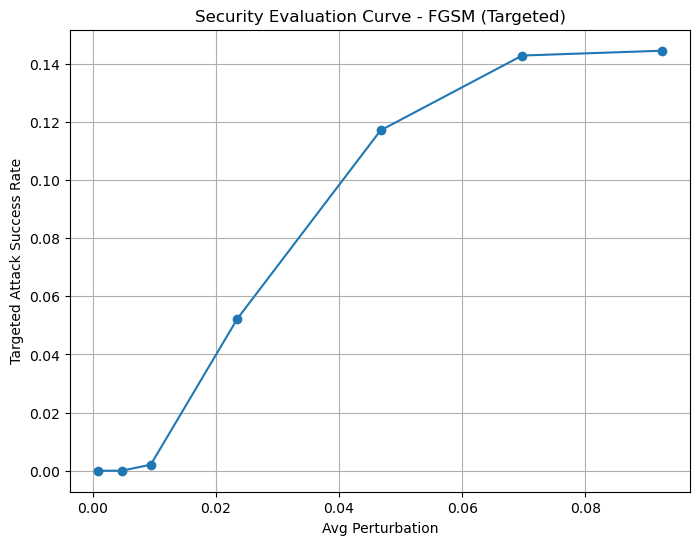
\includegraphics[width=0.65\textwidth]{images/evaluation_curve_fgsm_targeted.png}
                \caption{Security Evaluation Curve per FGSM Targeted. L'asse delle ascisse rappresenta la perturbazione media, mentre l'asse delle ordinate mostra la targeted success rate.}
                \label{fig:fgsm_targeted_curve}
            \end{figure}
            
            \noindent Come si osserva dalla Figura~\ref{fig:fgsm_targeted_curve}, l'efficacia dell'attacco cresce al crescere della perturbazione introdotta, ma in maniera piuttosto contenuta. L'attacco ottiene un successo massimo del 14.45\% per \(\epsilon = 0.1\), confermando che l’FGSM risulta inefficace per attacchi mirati a bassa perturbazione.
            
            \begin{table}[H]
                \centering
                \label{tab:fgsm_targeted}
                \begin{tabular}{c|c|c|c}
                    \toprule
                    \textbf{Epsilon} & \textbf{Perturbazione media} & \(\mathbf{L_\infty}\) & \textbf{Targeted Success Rate} \\
                    \midrule
                    0.001 & 0.0009 & 0.0010 & 0.00\% \\
                    0.005 & 0.0047 & 0.0050 & 0.00\% \\
                    0.010 & 0.0094 & 0.0100 & 0.21\% \\
                    0.025 & 0.0235 & 0.0250 & 5.23\% \\
                    0.050 & 0.0467 & 0.0500 & 11.71\% \\
                    0.075 & 0.0697 & 0.0750 & 14.29\% \\
                    0.100 & 0.0924 & 0.1000 & 14.45\% \\
                    \bottomrule
                \end{tabular}
                \caption{Risultati ottenuti con FGSM targeted.}
            \end{table}

        \subsection{Basic Iterative Method (Targeted)}
            Il \textit{Basic Iterative Method} (BIM) estende FGSM applicando la perturbazione in più passi di piccola entità. Nella modalità targeted, l’attacco forza l'immagine verso una classe obiettivo $y_{\text{target}}$ minimizzando la loss rispetto a tale classe. La formula ricorsiva del metodo è:
            
            \[
            x_t = x_{t-1} - \alpha \cdot \text{sign}\left( \nabla_x \mathcal{L}(h(x_{t-1}, w), y_{\text{target}}) \right)
            \]
            
            \noindent dove $\alpha = \epsilon / T$ rappresenta lo step size e $T$ è il numero totale di step.
            L'attacco  è stato valutato su un ampio spettro di valori del parametro \(\epsilon\), variando anche il numero massimo di iterazioni tra \texttt{5}, \texttt{10} e \texttt{20}. 
            
            \begin{figure}[H]
                \centering
                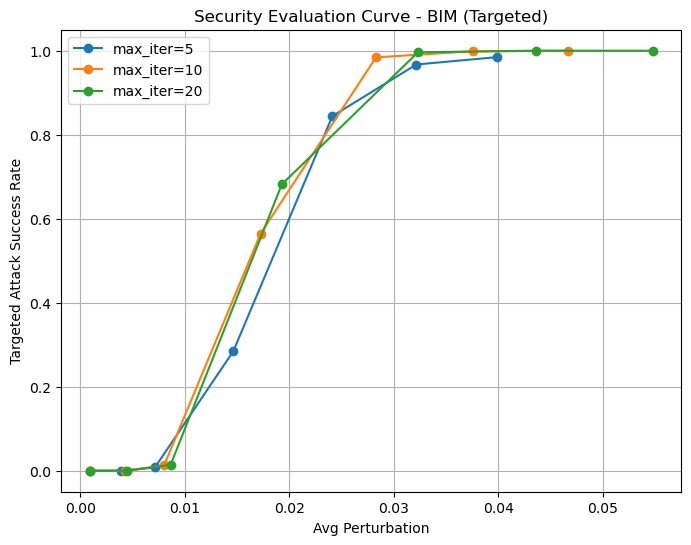
\includegraphics[width=0.75\textwidth]{images/evaluation_curve_bim_targeted.png}
                \caption{Security Evaluation Curve per l’attacco BIM in modalità targeted.}
                \label{fig:bim_targeted_curve}
            \end{figure}
            
            \noindent I risultati riportati in Figura~\ref{fig:bim_targeted_curve} mostrano un comportamento estremamente interessante: per valori bassi di \(\epsilon\) (\(\leq 0.005\)), l’attacco è inefficace indipendentemente dal numero di iterazioni, con un tasso di successo nullo. Ciò è dovuto al fatto che la distanza da percorrere per raggiungere una specifica classe bersaglio può richiedere modifiche più marcate rispetto al semplice inganno generico del classificatore. In questi casi, la rete neurale resiste bene a perturbazioni minime mirate.
            A partire da \(\epsilon = 0.01\), si inizia a osservare un lieve miglioramento, ma è solo con \(\epsilon \geq 0.025\) che l’attacco diventa significativamente efficace. In particolare, per \(\epsilon = 0.025\) e \texttt{max\_iter = 20}, il tasso di successo raggiunge il 68\%, crescendo poi rapidamente verso il 100\% con \(\epsilon = 0.075\) o superiore.
            Si nota inoltre come il numero di iterazioni gioca un ruolo cruciale: a parità di \(\epsilon\), passare da 5 a 20 iterazioni porta miglioramenti tangibili. Questo è coerente con la natura iterativa del BIM, che riesce a modellare gradualmente la perturbazione per renderla più efficace nel colpire la classe obiettivo.
            Infine, è importante osservare che l’alta efficacia dell’attacco non comporta necessariamente perturbazioni visivamente percepibili. Anche per \(\epsilon = 0.075\), la perturbazione media si aggira attorno a 0.04 (in scala normalizzata), dimostrando che l’avversario può ottenere una manipolazione mirata con alterazioni minime ma strategicamente dirette.

        \subsection{Projected Gradient Descent (Targeted)}
            Il \textit{Projected Gradient Descent} (PGD), nella modalità targeted, estende l’attacco BIM iterando piccoli passi verso la classe target e proiettando ad ogni passo l’immagine avversaria all’interno di una sfera $L\infty$ di raggio $\epsilon$ centrata sull’immagine originale:
            \[
            x_t = \Pi_\epsilon \left( x_{t-1} - \alpha \cdot \text{sign}( \nabla_x \mathcal{L}(h(x{t-1}, w), y_{\text{target}}) \right)
            \]
            
            \noindent dove $\Pi_\epsilon$ rappresenta la proiezione, $\alpha$ è lo step size definito come $\epsilon/5$ e $y_{\text{target}}$ è la classe desiderata.
            
            \begin{figure}[H]
                \centering
                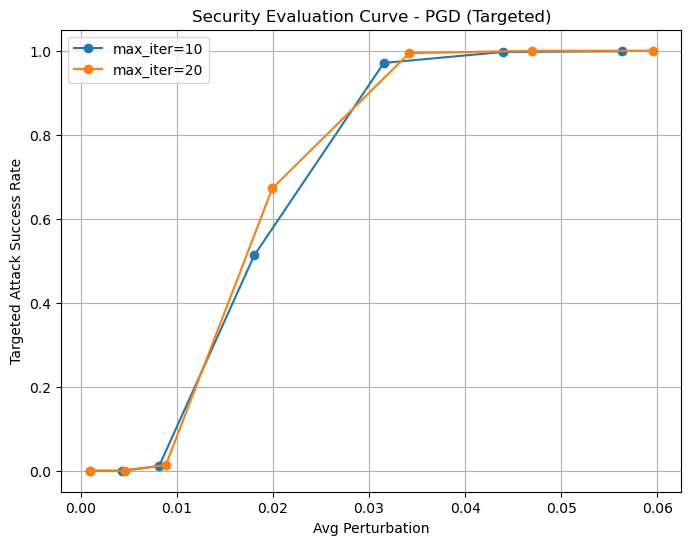
\includegraphics[width=0.75\textwidth]{images/evaluation_curve_pgd_targeted.png}
                \caption{Security Evaluation Curve per l’attacco PGD targeted, variando \texttt{max\_iter}.}
                \label{fig:pgd_targeted_curve}
            \end{figure}
            
            \noindent Come mostrato nella Figura~\ref{fig:pgd_targeted_curve}, PGD targeted è in grado di raggiungere un’elevata efficacia al crescere di \(\epsilon\), confermando la sua natura di attacco potente e controllabile. Per valori molto piccoli (\(\epsilon \leq 0.005\)), l'attacco fallisce nel condurre il classificatore verso la classe obiettivo, indipendentemente dal numero di iterazioni. Questo è un comportamento prevedibile, in quanto la distanza decisionale da colmare per passare a una classe specifica richiede modifiche più ampie rispetto al semplice errore di classificazione.
            Al crescere di \(\epsilon\), il successo aumenta in modo non lineare, si osserva infatti un punto di svolta attorno a \(\epsilon = 0.025\), dove il tasso di successo raggiunge il 50–67\%, e poi una rapida convergenza verso il 100\% già a \(\epsilon = 0.050\). L’impatto del numero di iterazioni è visibile ma limitato: 20 iterazioni permettono un attacco più efficace rispetto a 10 iterazioni, soprattutto nelle fasce intermedie di perturbazione.
            È interessante notare che l’attacco riesce a raggiungere un tasso di successo pressoché completo mantenendo una media di perturbazione ancora accettabile (\textasciitilde{}0.05), suggerendo che PGD sia in grado di costruire perturbazioni mirate ed efficaci, pur restando all’interno di soglie realistiche di impercettibilità visiva.
            Questa capacità di bilanciare efficacia e controllo fine del rumore rende PGD uno degli attacchi targeted più pericolosi tra quelli testati.

    \section{Carlini-Wagner L2 (Targeted)}
        L’attacco Carlini \& Wagner (CW) è noto per essere uno dei più efficaci nel contesto degli attacchi avversari, soprattutto nella modalità \textit{targeted}, dove l’obiettivo è forzare il modello a classificare un input come una specifica classe scelta. In questa sezione è stato implementato l’attacco CW-L2 in modalità targeted contro il modello NN1, variando i principali iperparametri di attacco per studiarne l’influenza sulla percentuale di successo e sull’entità della perturbazione.

        \subsection{Setup}
            Sono stati selezionati casualmente 20 campioni dal test set. Per ciascuno di essi è stata definita una classe target ciclica (\texttt{target = (label + 1) \% num\_classes}). Gli attacchi sono stati condotti variando:
            
            \begin{itemize}
              \item il \textbf{learning rate} ($lr \in \{0.01, 0.1\}$),
              \item il numero massimo di iterazioni ($max\_iter \in \{1, 10, 20\}$),
              \item la costante iniziale di bilanciamento tra obiettivo e perturbazione ($init\_const \in \{0.01, 0.1\}$).
            \end{itemize}

        \subsection{Risultati e Analisi}
            Il primo grafico (\autoref{fig:cw_l2_acc}) mostra l'\textbf{accuratezza targeted} in funzione del numero di iterazioni per diverse combinazioni di iperparametri. Si osserva chiaramente che:
                \begin{itemize}
                  \item L’aumento di \texttt{max\_iter} migliora significativamente il successo dell’attacco, a condizione che la costante iniziale non sia troppo bassa.
                  
                  \item La combinazione \texttt{lr=0.1} e \texttt{init\_const=0.1} consente di raggiungere il 100\% di successo già con sole 10 iterazioni, segno di una forte efficacia, ma anche di un possibile overfitting sulle immagini specifiche.
                \end{itemize}
            
            \begin{figure}[H]
                \centering
                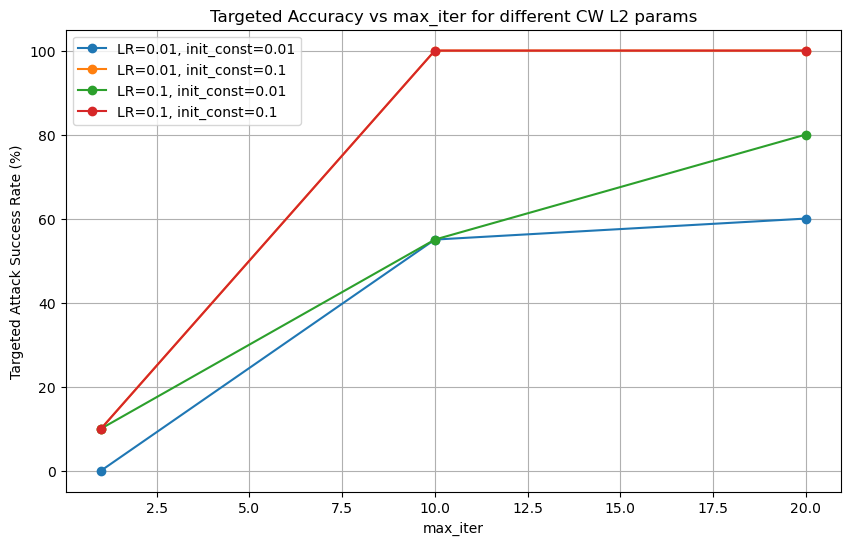
\includegraphics[width=0.75\textwidth]{images/cw_L2_accuracy_vs_maxiter.png}
                \caption{Targeted Attack Success Rate vs max\_iter per diverse combinazioni di parametri CW-L2}
                \label{fig:cw_l2_acc}
            \end{figure}
            
            \noindent Il secondo grafico (\autoref{fig:cw_l2_pert}) mostra l'\textbf{entità media della perturbazione} in norma $L_2$.
            In generale:
                \begin{itemize}
                  \item Le combinazioni con $init\_const=0.1$ inducono perturbazioni sensibilmente più alte, a discapito della stealthiness, ma a vantaggio della precisione.
                  
                  \item Le configurazioni con $lr=0.01$ mantengono perturbazioni più contenute, ma spesso richiedono più iterazioni per ottenere alti tassi di successo.
                \end{itemize}
            
            \begin{figure}[H]
                \centering
                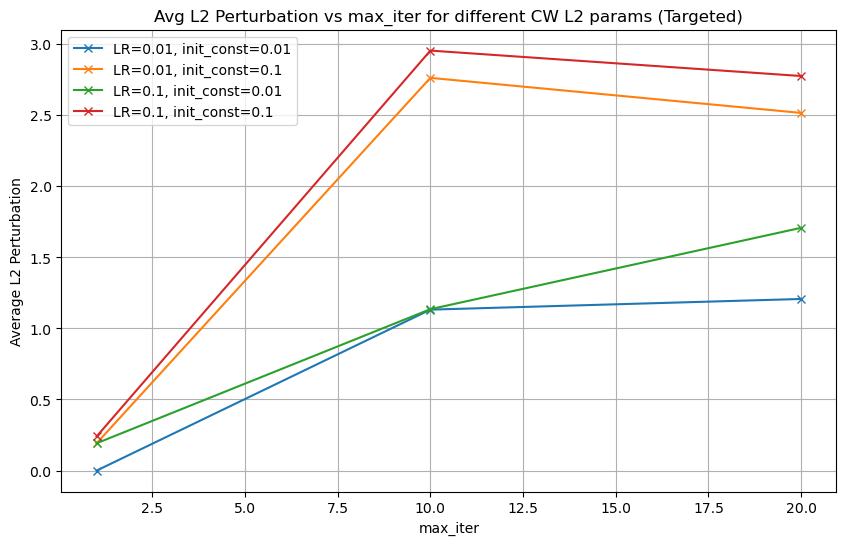
\includegraphics[width=0.75\textwidth]{images/cw_L2_perturbation_vs_maxiter.png}
                \caption{Average L2 Perturbation vs max\_iter per diverse combinazioni di parametri CW-L2}
                \label{fig:cw_l2_pert}
            \end{figure}
            
            \noindent Infine, la \textbf{Security Evaluation Curve} (\autoref{fig:cw_l2_sec}) mostra il trade-off tra efficacia e visibilità dell’attacco: all’aumentare della norma $L_2$, la percentuale di successo cresce in modo monotono, indicando una correlazione positiva tra aggressività e capacità di forzare la classificazione.
            
            \begin{figure}[H]
                \centering
                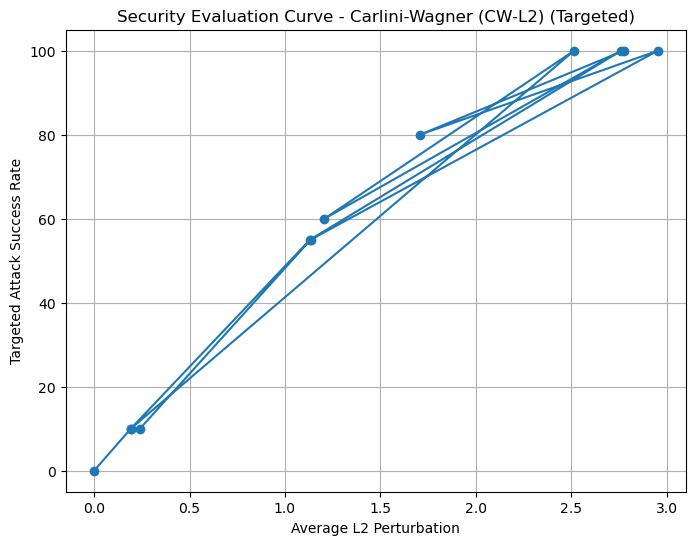
\includegraphics[width=0.65\textwidth]{images/cw_L2_security_curve.png}
                \caption{Security Evaluation Curve - Carlini \& Wagner (CW-L2) in modalità targeted}
                \label{fig:cw_l2_sec}
            \end{figure}

        \subsection{Osservazioni}
            Il raggiungimento del 100\% di successo in molte configurazioni non è anomalo per questo tipo di attacco, ma va interpretato con cautela: il CW-L2 è un attacco ottimizzativo potente, ma lavora su un piccolo subset di dati (20 immagini) e sfrutta conoscenza completa del modello. Di conseguenza, i risultati riflettono un'efficacia teorica elevata, che potrebbe ridursi in scenari reali o su modelli differenti.

    \section{Carlini-Wagner $L\infty$ (Targeted)}
        In questo esperimento abbiamo valutato l’efficacia dell’attacco \textit{Carlini-Wagner $L\infty$} in modalità \textit{targeted}, utilizzando il modello NN1 come rete bersaglio. Sono stati testati diversi valori per i principali iperparametri dell’attacco: \texttt{learning\_rate} $\in \{0.01, 0.1\}$, \texttt{initial\_const} $\in \{0.01, 0.1\}$, e \texttt{max\_iter} $\in \{1, 10, 20\}$. L’obiettivo era osservare come la variazione di tali parametri influenzasse la \textit{Targeted Attack Success Rate} e la dimensione della perturbazione media generata.
        
        \subsection{Risultati sperimentali}
            I risultati sperimentali mostrano che l’attacco Carlini-Wagner in modalità \textit{targeted} con norma $L\infty$ non ha prodotto alcun successo nel forzare la rete NN1 a classificare gli esempi avversari nella classe obiettivo, difatti in tutte le configurazioni testate, il tasso di successo è rimasto pari a $0\%$. Sebbene in alcune impostazioni siano state riscontrate perturbazioni visibili (con norma $L\infty$ fino a 0.0999), queste non si sono rivelate sufficienti a influenzare le decisioni del classificatore nella direzione desiderata.
            Tale risultato non implica necessariamente che l’attacco CW-$L\infty$ sia inefficace in senso assoluto. Al contrario, come evidenziato nel lavoro originale di Carlini e Wagner, l’attacco richiede in genere un numero molto elevato di iterazioni (spesso tra le 100 e le 1000) per ottimizzare efficacemente la perturbazione nella metrica $L\infty$ in contesto \textit{targeted}. Nel nostro caso, per motivi legati ai vincoli computazionali e alla disponibilità di tempo, abbiamo limitato il numero di iterazioni a $\{1, 10, 20\}$, valore che si è rivelato insufficiente per ottenere risultati significativi.
            È importante sottolineare che l’attacco CW-$L\infty$ è strutturato e potenzialmente molto potente, ma la sua efficacia dipende fortemente da un tuning accurato dei parametri e da un budget computazionale elevato. In assenza di tali condizioni, l’ottimizzazione risulta incompleta e incapace di generare perturbazioni che raggiungano l’obiettivo di classificazione imposto. In questo contesto, l'apparente fallimento dell'attacco è da attribuirsi principalmente a una configurazione sperimentale conservativa e non a una limitazione teorica dell'approccio stesso.
            
    \section{Confronto tra gli Attacchi Targeted}
        I risultati ottenuti mostrano una marcata differenza in termini di efficacia tra gli attacchi targeted analizzati. Gli attacchi iterativi come BIM e PGD si sono dimostrati estremamente efficaci nel forzare la rete a classificare le immagini secondo le etichette obiettivo, raggiungendo tassi di successo superiori al 99\% con valori di $\epsilon$ moderati e un numero di iterazioni sufficientemente alto.
        Al contrario, FGSM targeted ha mostrato un'efficacia molto limitata: essendo un attacco single-step, le perturbazioni risultano troppo deboli per influenzare il comportamento del classificatore verso una classe specifica.
        Il metodo Carlini-Wagner, pur essendo noto per la sua efficacia in modalità non-targeted, non ha prodotto risultati utili nella configurazione targeted sul nostro campione. Questo è probabilmente dovuto alla complessità del loss utilizzato, alla difficoltà di ottimizzazione in spazi ad alta dimensione e alla dimensione ridotta del test set.
    \chapter{Verifica della Trasferibilità degli Attacchi}
    In questo capitolo analizziamo la trasferibilità degli adversarial attacks, ovvero la loro capacità di ingannare modelli differenti da quello bersaglio utilizzato per la generazione. Questa proprietà è particolarmente pericolosa in ambito di sicurezza, poiché consente a un attaccante di compromettere un sistema anche senza conoscere la sua architettura interna, basandosi solo su un modello sostitutivo.
    Per valutare la trasferibilità, abbiamo introdotto un secondo classificatore, denominato \textbf{NN2}, basato sull’architettura \textit{ResNet50}, pre-addestrato sul dataset VGG-Face2. Il modello è stato caricato con pesi ottimizzati (fine-tuning) corrispondenti a 8631 identità. La rete NN2 differisce in modo sostanziale da NN1 (modello usato per generare gli attacchi), offrendo quindi un contesto adatto per una valutazione realistica della robustezza cross-architettura.

    \section{Trasferibilità: Aspetti Teorici}
        La trasferibilità degli attacchi adversarial rappresenta uno dei fenomeni più rilevanti e preoccupanti nel contesto della sicurezza dei modelli di deep learning. Studi empirici e teorici hanno mostrato che input modificati per ingannare un determinato modello possono spesso mantenere la loro efficacia anche su modelli con architetture diverse o parametri differenti. Questo comportamento, noto come \textit{cross-model transferability}, si manifesta con particolare evidenza nei cosiddetti attacchi \textit{error-generic}, che mirano a ottenere una classificazione errata, indipendentemente dalla classe di destinazione.
        Il meccanismo alla base di questa proprietà è legato alla similarità strutturale tra le rappresentazioni interne apprese da modelli diversi, specialmente se addestrati sullo stesso dominio. Di conseguenza, le perturbazioni che alterano i confini decisionali in un modello possono avere un effetto simile anche su un altro. In contesti reali, ciò significa che un attaccante può generare un attacco utilizzando un modello accessibile (\textit{surrogate}) e poi utilizzarlo con successo contro un sistema chiuso o sconosciuto, senza la necessità di conoscere la sua struttura o i suoi pesi.
        La probabilità di successo della trasferibilità dipende da diversi fattori, tra cui l’intensità della perturbazione, la somiglianza tra le architetture e il tipo di attacco utilizzato. Gli attacchi targeted, ad esempio, richiedono che l’input venga classificato come una specifica classe bersaglio e tendono quindi a trasferirsi meno efficacemente rispetto a quelli non mirati. Tuttavia, anche in questi casi sono stati osservati effetti non trascurabili, soprattutto con architetture con strutture latenti simili.
        Nel contesto del nostro progetto, la valutazione della trasferibilità consente di stimare l’efficacia reale degli attacchi generati su NN1 quando applicati a NN2, fornendo così una misura indiretta della pericolosità di tali perturbazioni in uno scenario di tipo black-box.
    
    \section{Implementazione del Modello NN2}
        Il modello NN2 è stato caricato utilizzando la libreria \texttt{torchvision} e i pesi pre-addestrati sono stati caricati da un file \texttt{resnet50\_ft\_weight.pkl}. Prima di passare i dati in input alla rete, è stato necessario replicare il preprocessing previsto per il training originale:
            \begin{itemize}
              \item Le immagini, originariamente normalizzate in $[-1, 1]$, sono state scalate nel range $[0, 255]$
              
              \item I canali RGB sono stati convertiti in BGR
              
              \item È stata sottratta la media per canale usata durante il fine-tuning (\texttt{mean\_bgr} = [91.4953, 103.8827, 131.0912])
              
              \item Le immagini sono state ridimensionate da $160 \times 160$ a $224 \times 224$ pixel, come richiesto da ResNet50
            \end{itemize}
    
    \section{Obiettivo dell’Analisi}
        L’obiettivo di questo capitolo è verificare se gli \textit{adversarial examples} generati su NN1 sono in grado di compromettere anche NN2. Questo viene valutato riproducendo le predizioni di NN2 sugli stessi campioni avversari (salvati da attacchi come FGSM, BIM, PGD, ecc.) e confrontando le etichette predette con quelle corrette.
        Per mantenere la coerenza tra le classi, è stata implementata una procedura di mappatura tra le etichette predette da NN2 e quelle usate durante la generazione su NN1. In fase di test, sono state mascherate le uscite della rete NN2 per considerare solo le classi presenti nel test set, in modo da evitare interferenze da identità non presenti.
        Nei paragrafi successivi vengono presentati i risultati sperimentali relativi alla trasferibilità di ciascun attacco error-generic e poi in seguito error-specific.

    \section{Trasferibilità dell'attacco FGSM Non-Targeted}
        L'attacco \textbf{FGSM non-targeted}, generato sulla rete NN1, è stato valutato per verificarne la \textit{trasferibilità} verso il classificatore NN2 (ResNet50). In questo caso, l’obiettivo delle perturbazioni non è forzare una classe specifica, ma semplicemente indurre una classificazione errata. L’efficacia della trasferibilità è stata misurata tramite l’accuratezza residua di NN2 nel classificare correttamente i campioni avversari.
        Il grafico in Figura~\ref{fig:fgsm_untargeted_transfer} mostra il comportamento dell'accuratezza del modello NN2 rispetto alla \textit{perturbazione media} introdotta, misurata in norma L$\infty$.
        
        \begin{figure}[H]
          \centering
          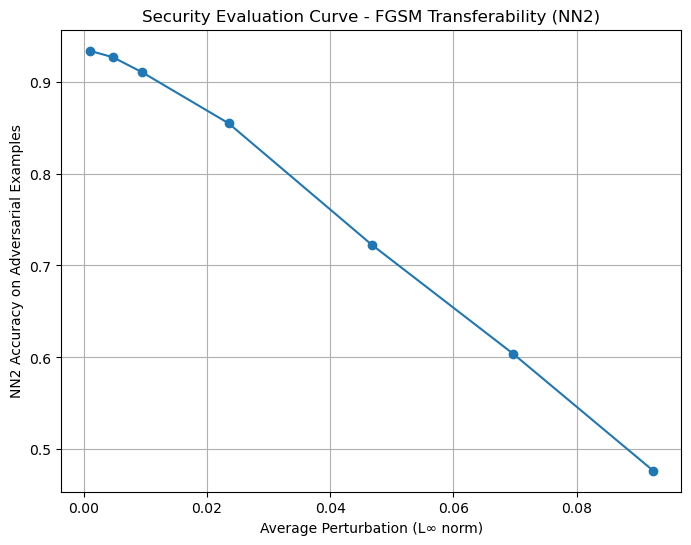
\includegraphics[width=0.7\textwidth]{images/untargFGSMtrasf.png}
          \caption{Security Evaluation Curve - FGSM Transferability (Non-Targeted, NN2)}
          \label{fig:fgsm_untargeted_transfer}
        \end{figure}

        \subsection{Osservazioni}
            I risultati numerici confermano un degrado progressivo delle prestazioni di NN2 all’aumentare della perturbazione:
                \begin{center}
                    \begin{tabular}{ccc}
                        \toprule
                        \textbf{Perturbazione media (L$_1$)} & \textbf{L$\infty$} & \textbf{Accuracy (\%)} \\
                        \midrule
                        0.0009 & 0.0010 & 93.36 \\
                        0.0047 & 0.0050 & 92.65 \\
                        0.0094 & 0.0100 & 91.03 \\
                        0.0235 & 0.0250 & 85.47 \\
                        0.0467 & 0.0500 & 72.26 \\
                        0.0697 & 0.0750 & 60.38 \\
                        0.0924 & 0.1000 & 47.67 \\
                        \bottomrule
                    \end{tabular}
                \end{center}

        \subsection{Analisi}
            L'attacco FGSM non-targeted mostra un'evidente capacità di trasferirsi da NN1 a NN2. Anche con perturbazioni di modesta entità (ad esempio L$\infty=0.025$), l'accuratezza del modello di destinazione si riduce significativamente. Con un'intensità massima (L$\infty=0.1$), la rete ResNet50 commette errori su oltre metà dei campioni avversari, dimostrando la vulnerabilità del sistema anche in uno scenario completamente black-box.
            Questo comportamento conferma quanto ampiamente documentato in letteratura, ovvero che gli attacchi \textit{non-targeted}, meno vincolati rispetto a quelli \textit{targeted}, tendono a produrre perturbazioni più generiche, in grado di colpire modelli con strutture interne differenti. La loro semplicità di generazione li rende strumenti particolarmente pericolosi in contesti in cui l’attaccante non ha accesso diretto al modello bersaglio.

    \section{Trasferibilità dell'attacco BIM Non-Targeted}
        L'attacco \textbf{Basic Iterative Method} (BIM), generato a partire dal modello NN1, è stato analizzato per verificarne la \textit{trasferibilità} verso NN2. A differenza di FGSM, BIM applica la perturbazione in modo iterativo, accumulando modifiche lungo la direzione del gradiente a ogni passo. Questo lo rende un attacco più preciso, ma potenzialmente anche più overfittato al modello di origine. L’obiettivo di questa analisi è determinare se tale maggiore precisione comprometta la capacità di trasferirsi verso architetture differenti.
        Nel grafico di Figura~\ref{fig:bim_transfer} è riportata la curva di accuratezza residua di NN2 rispetto alla perturbazione media, considerando tre configurazioni di attacco (5, 10 e 20 iterazioni) a parità di $\epsilon$ massimo.

        \begin{figure}[H]
          \centering
          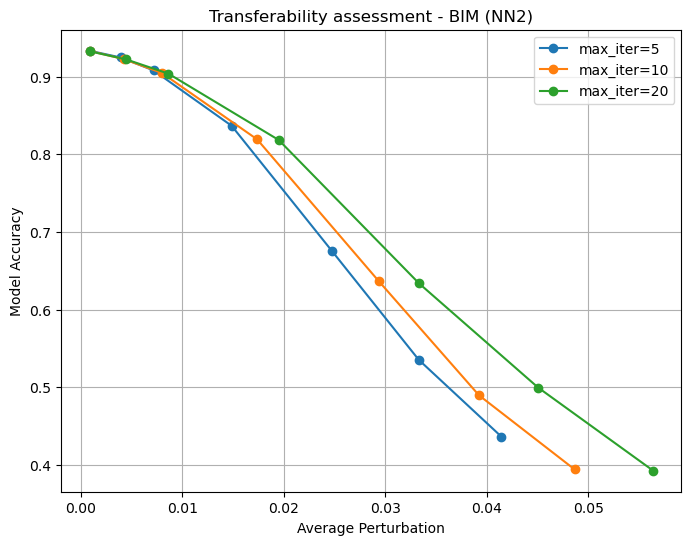
\includegraphics[width=0.7\textwidth]{images/untargBIMtrasf.png}
          \caption{Transferability assessment - BIM (NN2)}
          \label{fig:bim_transfer}
        \end{figure}

        \subsection{Osservazioni}
            La tabella seguente mostra i valori ottenuti per alcune delle principali configurazioni testate. Le perturbazioni sono espresse in norma L$\infty$ media, mentre l’accuratezza riflette la percentuale di predizioni corrette effettuate da NN2:
                \begin{center}
                    \begin{tabular}{cccc}
                        \toprule
                        \textbf{max\_iter} & \textbf{Perturbazione media} & \textbf{L$\infty$} & \textbf{Accuracy (\%)} \\
                        \midrule
                        5  & 0.0414 & 0.1000 & 43.65 \\
                        10 & 0.0487 & 0.1000 & 39.41 \\
                        20 & 0.0564 & 0.1000 & 39.24 \\
                        \bottomrule
                    \end{tabular}
                \end{center}

        \subsection{Analisi}
            I risultati mostrano che, come per FGSM, anche l’attacco BIM è in grado di trasferirsi da NN1 a NN2 in modo efficace. L’aumento del numero di iterazioni comporta una perturbazione media più ampia, ma la differenza di accuratezza residua tra $max\_iter = 10$ e $20$ è marginale, suggerendo una saturazione dell'effetto dopo un certo numero di passi.
            Con L$\infty = 0.1$ e perturbazioni medie comprese tra 0.04 e 0.056, l’accuratezza di NN2 scende sotto il 40\%, confermando la vulnerabilità cross-architettura del modello anche di fronte ad attacchi iterativi.
            Questi risultati indicano che, nonostante la maggiore specificità delle perturbazioni rispetto a FGSM, BIM mantiene un alto grado di trasferibilità, in particolare nelle configurazioni a media iterazione. Ciò lo rende una tecnica pericolosa anche in contesti black-box, dove l'attaccante può solo stimare la rete bersaglio.

    \section{Trasferibilità dell'attacco PGD Non-Targeted}
        L’attacco \textbf{Projected Gradient Descent} (PGD) rappresenta una generalizzazione iterativa del metodo FGSM, con proiezione dentro la $\epsilon$-ball. È considerato uno degli attacchi più robusti in letteratura ed è comunemente utilizzato come benchmark per la valutazione della resilienza dei modelli. In questo esperimento, sono state generate perturbazioni su NN1 e successivamente testate sulla rete NN2 per valutare la \textit{trasferibilità} cross-architettura.
        La Figura~\ref{fig:pgd_transfer} riporta l’accuratezza del modello NN2 rispetto alla \textit{perturbazione media} introdotta, per due configurazioni di attacco: \texttt{max\_iter=10} e \texttt{max\_iter=20}.
        
        \begin{figure}[H]
          \centering
          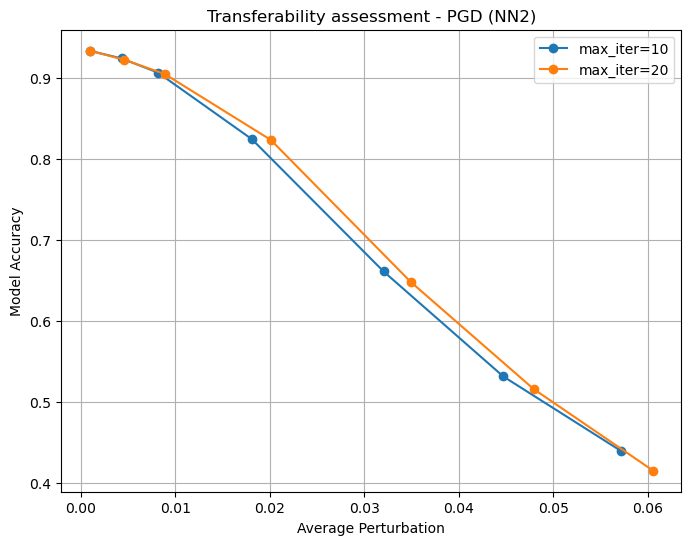
\includegraphics[width=0.7\textwidth]{images/untargPGDtrasf.png}
          \caption{Transferability assessment - PGD (NN2)}
          \label{fig:pgd_transfer}
        \end{figure}

        \subsection{Osservazioni}
            La tabella seguente riassume i risultati per i due setting di iterazioni. Come per BIM, è evidente un effetto di saturazione per iterazioni elevate, ma le prestazioni restano inferiori rispetto al test su immagini pulite:
                \begin{center}
                    \begin{tabular}{cccc}
                        \toprule
                        \textbf{max\_iter} & \textbf{Perturbazione media} & \textbf{L$\infty$} & \textbf{Accuracy (\%)} \\
                        \midrule
                        10 & 0.0009 & 0.0010 & 93.31 \\
                        10 & 0.0043 & 0.0050 & 92.36 \\
                        10 & 0.0082 & 0.0100 & 90.61 \\
                        10 & 0.0181 & 0.0250 & 82.39 \\
                        10 & 0.0320 & 0.0500 & 66.07 \\
                        10 & 0.0447 & 0.0750 & 53.11 \\
                        10 & 0.0571 & 0.1000 & 43.94 \\
                        \midrule
                        20 & 0.0010 & 0.0010 & 93.31 \\
                        20 & 0.0046 & 0.0050 & 92.19 \\
                        20 & 0.0089 & 0.0100 & 90.45 \\
                        20 & 0.0201 & 0.0250 & 82.31 \\
                        20 & 0.0349 & 0.0500 & 64.78 \\
                        20 & 0.0479 & 0.0750 & 51.58 \\
                        20 & 0.0606 & 0.1000 & 41.49 \\
                        \bottomrule
                    \end{tabular}
                \end{center}

        \subsection{Analisi}
            L’attacco PGD si dimostra altamente trasferibile verso NN2.
            Analizzando i dati nel dettaglio, si osserva che per $\epsilon \leq 0.005$, l’accuratezza di NN2 resta pressoché invariata sopra il 92\%, indipendentemente dal numero di iterazioni. In questo intervallo, l’effetto dell’attacco è minimo: la perturbazione media è troppo contenuta per produrre uno spostamento significativo nella distribuzione delle attivazioni interne.
            Superata la soglia di $\epsilon = 0.01$, l’impatto dell’attacco diventa più marcato: a $\epsilon = 0.025$, l’accuratezza scende all’82.39\% (con 10 iterazioni) e 82.31\% (con 20 iterazioni), mostrando una convergenza dei due setting e un iniziale effetto di saturazione. Ciò indica che il numero di iterazioni incide poco e che il limite dell'efficacia inizia a dipendere principalmente dal budget di perturbazione.
            Nella fascia intermedia ($\epsilon$ tra 0.05 e 0.075), l’effetto del numero di iterazioni inizia a emergere: si passa dal 66.07\% (iter=10) al 64.78\% (iter=20) e dal 53.11\% al 51.58\%, mostrando che iterazioni aggiuntive consentono una minima ma sistematica erosione delle performance del modello.
            A $\epsilon = 0.1$, entrambi i setting raggiungono il picco massimo di distorsione consentita, con perturbazioni medie pari a circa 0.057–0.060. L’accuratezza precipita rispettivamente al 43.94\% e 41.49\%, confermando che l’attacco è in grado di colpire la rete anche in profondità, inducendo errori sistematici. L’effetto di \texttt{max\_iter} tende a stabilizzarsi, segno che la strategia ha raggiunto la sua piena capacità d’impatto entro i 20 passi.
            Nel complesso, PGD dimostra un’ottima scalabilità e trasferibilità, con un comportamento coerente lungo tutta la curva e un degrado delle prestazioni che segue fedelmente l’intensità della perturbazione.
            Questi risultati consolidano PGD come una minaccia concreta anche in scenari black-box, grazie alla sua capacità di generare perturbazioni sufficientemente generiche da ingannare architetture differenti.

    \section{Trasferibilità dell'attacco DeepFool Non-Targeted}
        L'attacco \textbf{DeepFool} si basa su un approccio iterativo che mira a trovare la minima perturbazione possibile capace di condurre l'immagine oltre il confine decisionale del classificatore. A differenza degli altri metodi analizzati, DeepFool non impone vincoli espliciti sulla norma della perturbazione, ma ottimizza direttamente la distanza nel dominio delle decisioni. In questo esperimento, l’attacco è stato generato su NN1 e valutato su NN2 per stimare la capacità di trasferimento di perturbazioni minimali.
        Il test è stato condotto su un sottoinsieme di soli 10 campioni (a causa della complessità computazionale dell’attacco), selezionati in modo da garantire eterogeneità nelle classi di appartenenza.
        La Figura~\ref{fig:deepfool_transfer} mostra il singolo punto sperimentale ottenuto, rappresentante l’accuratezza di NN2 rispetto alla perturbazione media introdotta.
        
        \begin{figure}[H]
          \centering
          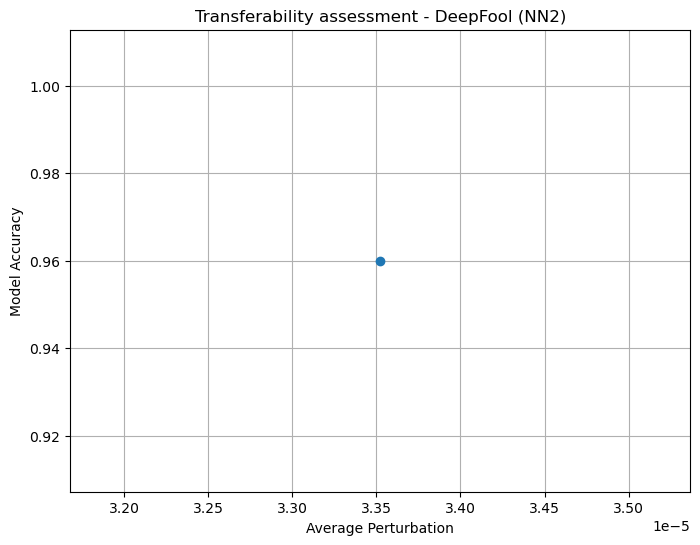
\includegraphics[width=0.65\textwidth]{images/untargDFtrasf.png}
          \caption{Transferability assessment - DeepFool (NN2).}
          \label{fig:deepfool_transfer}
        \end{figure}

        \subsection{Osservazioni}
            \noindent L’accuratezza di NN2 sugli esempi avversari generati da DeepFool si attesta al 96\%, suggerendo che la maggior parte delle predizioni resta corretta. La perturbazione media risulta estremamente bassa ($\sim 3.35 \times 10^{-5}$), mentre la norma massima L$\infty$ rilevata è pari a 0.0135. Questi valori confermano che le modifiche apportate alle immagini sono minime e spesso impercettibili anche da parte del modello ricevente.
            È importante notare che DeepFool ha lo scopo di generare perturbazioni di minima entità piuttosto che massimizzare l’effetto avversario. Per questo motivo, la bassa efficacia in termini di trasferibilità è attesa. Inoltre, il fatto che l’attacco sia costruito esplicitamente per un solo classificatore (NN1), senza sfruttare regolarizzazioni che ne aumentino la generalizzabilità, contribuisce alla bassa riuscita su NN2.

            \begin{center}
                \begin{tabular}{cccc}
                    \toprule
                    \textbf{Epsilon} & \textbf{Perturbazione media} & \textbf{L$\infty$} & \textbf{Accuracy (\%)} \\
                    \midrule
                    0.020 & 0.0000 & 0.0135 & 96.00 \\
                    \bottomrule
                \end{tabular}
            \end{center}

        \subsection{Analisi}
            I risultati confermano che, pur essendo un attacco molto efficace nel contesto white-box, DeepFool si dimostra scarsamente trasferibile. La sua forza risiede nella precisione geometrica nel manipolare la decision boundary del modello su cui viene eseguito; tuttavia, questa precisione lo rende anche poco adatto a scenari black-box, dove le peculiarità della rete bersaglio differiscono significativamente da quelle del generatore.
            In conclusione, DeepFool rappresenta un attacco ideale per valutazioni puntuali e teoriche, ma non costituisce una minaccia concreta in contesti in cui l’attaccante non ha accesso diretto alla rete obiettivo.

    \section{Trasferibilità dell'attacco Carlini-Wagner Non-Targeted L$\infty$}
        L’attacco \textbf{Carlini-Wagner} (CW) è noto per la sua efficacia nel produrre perturbazioni quasi invisibili e per la sua formulazione basata sull’ottimizzazione vincolata. In questo esperimento, sono state generate perturbazioni su NN1 con diverse configurazioni di parametri e successivamente testate su NN2 per valutare la \textit{trasferibilità}.
        Le Figure~\ref{fig:cw_transfer1},~\ref{fig:cw_transfer2} e~\ref{fig:cw_transfer3} illustrano rispettivamente:
        \begin{itemize}
          \item la curva di accuratezza di NN2 rispetto alla perturbazione media introdotta;
          
          \item la variazione della perturbazione media rispetto a \texttt{max\_iter}, per ciascuna configurazione;
          
          \item l’accuratezza del modello in funzione di \texttt{max\_iter}, per diverse coppie \texttt{lr}/\texttt{init\_const}.
        \end{itemize}

        \begin{figure}[H]
          \centering
          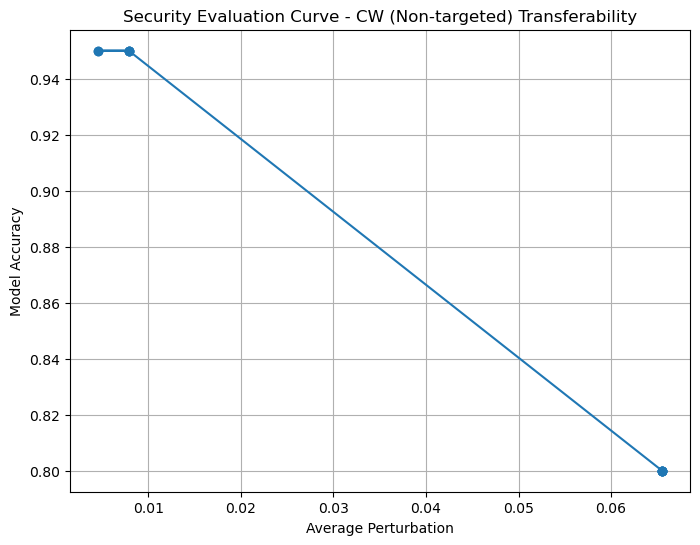
\includegraphics[width=0.7\textwidth]{images/cwtras3.png}
          \caption{Security Evaluation Curve - CW L$\infty$ (Non-targeted) Transferability}
          \label{fig:cw_transfer1}
        \end{figure}
        
        \begin{figure}[H]
          \centering
          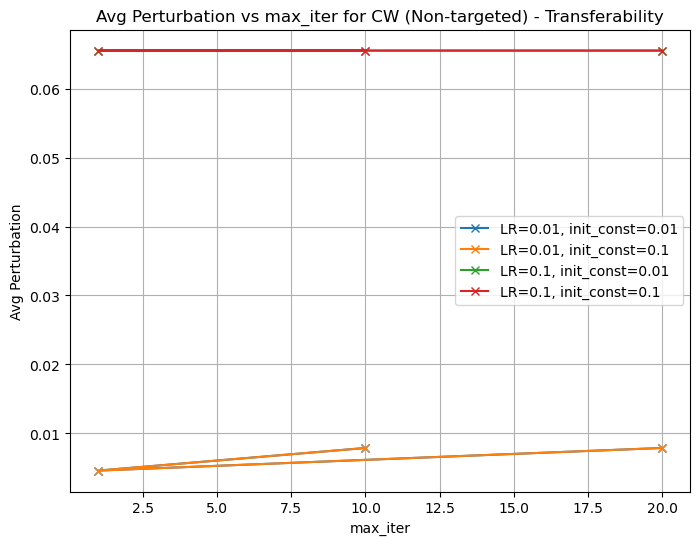
\includegraphics[width=0.7\textwidth]{images/cwtras2.png}
          \caption{Avg Perturbation vs \texttt{max\_iter} per CW L$\infty$ (Non-targeted)}
          \label{fig:cw_transfer2}
        \end{figure}
        
        \begin{figure}[H]
          \centering
          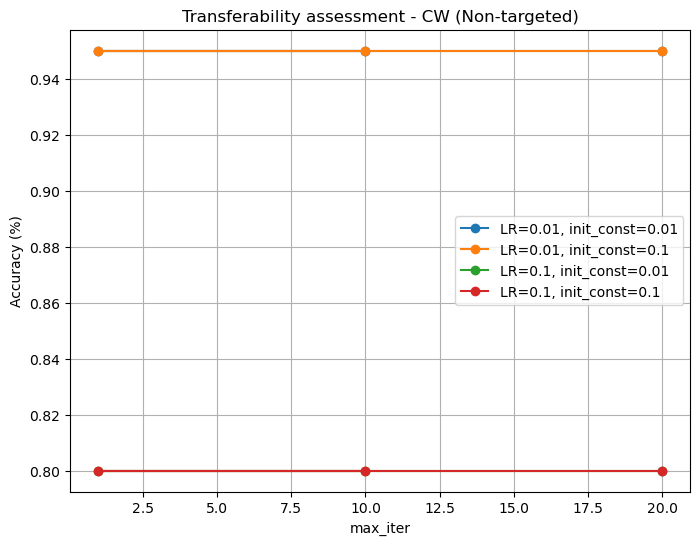
\includegraphics[width=0.7\textwidth]{images/cwtras1.png}
          \caption{Transferability assessment - CW L$\infty$ (Non-targeted)}
          \label{fig:cw_transfer3}
        \end{figure}

        \subsection{Osservazioni}
            I risultati ottenuti indicano un comportamento fortemente dipendente dal valore del learning rate.
            In particolare:
                \begin{itemize}
                  \item Per \texttt{lr = 0.01}, indipendentemente da \texttt{init\_const} e \texttt{max\_iter}, le perturbazioni risultano modeste ($\sim$0.0046--0.0079) e l’accuratezza di NN2 si mantiene elevata ($\sim$95\%).
                  
                  \item Per \texttt{lr = 0.1}, invece, la perturbazione media raggiunge $\sim$0.0655 con $L\infty \sim 0.0999$, producendo un drastico calo dell’accuratezza di NN2 (fino all’80\%).
                \end{itemize}
            
            \noindent I valori numerici sono riassunti nella tabella seguente:
                \begin{center}
                    \begin{tabular}{cccccc}
                        \toprule
                        \textbf{lr} & \textbf{max\_iter} & \textbf{init\_const} & \textbf{Pert. media} & \textbf{L$\infty$} & \textbf{Accuracy (\%)} \\
                        \midrule
                        0.01 & 1  & 0.01 & 0.0046 & 0.0100 & 95.00 \\
                        0.01 & 1  & 0.1  & 0.0046 & 0.0100 & 95.00 \\
                        0.01 & 10 & 0.01 & 0.0079 & 0.0200 & 95.00 \\
                        0.01 & 10 & 0.1  & 0.0079 & 0.0200 & 95.00 \\
                        0.01 & 20 & 0.01 & 0.0079 & 0.0200 & 95.00 \\
                        0.01 & 20 & 0.1  & 0.0079 & 0.0200 & 95.00 \\
                        0.1  & 1  & 0.01 & 0.0655 & 0.0999 & 80.00 \\
                        0.1  & 1  & 0.1  & 0.0655 & 0.0999 & 80.00 \\
                        0.1  & 10 & 0.01 & 0.0655 & 0.0999 & 80.00 \\
                        0.1  & 10 & 0.1  & 0.0655 & 0.0999 & 80.00 \\
                        0.1  & 20 & 0.01 & 0.0655 & 0.0999 & 80.00 \\
                        0.1  & 20 & 0.1  & 0.0655 & 0.0999 & 80.00 \\
                        \bottomrule
                    \end{tabular}
                \end{center}

        \subsection{Analisi}
            L’attacco CW non-targeted mostra una buona trasferibilità solo in presenza di un tasso di apprendimento elevato (\texttt{lr = 0.1}), che consente di superare una soglia di perturbazione tale da compromettere efficacemente NN2. Al contrario, per \texttt{lr = 0.01}, le perturbazioni restano contenute e altamente specifiche per NN1, riducendo l’efficacia in trasferimento.
            Questi risultati confermano che, sebbene CW sia potente in contesti white-box, la sua efficacia in black-box è fortemente condizionata dai parametri di ottimizzazione. Inoltre, la stabilità delle metriche tra diverse configurazioni di \texttt{init\_const} evidenzia come sia il learning rate a dominare il comportamento del trasferimento in questo scenario.

    \section{Trasferibilità dell'attacco Carlini-Wagner L$2$ (Non-targeted)}
        Per l'esperimento è stato utilizzato l'attacco Carlini-Wagner nella variante $L2$ non-targeted, valutando diverse combinazioni dei parametri: \texttt{learning\_rate} $\in \{0.01, 0.1\}$, \texttt{initial\_const} $\in \{0.01, 0.1\}$ e \texttt{max\_iter} $\in \{1, 10, 20\}$. I risultati sono riportati nei grafici in Figura~\ref{fig:cw_untarg_l2_acc}, \ref{fig:cw_untarg_l2_pert} e \ref{fig:cw_untarg_l2_sec}.
        
        \begin{figure}[H]
            \centering
            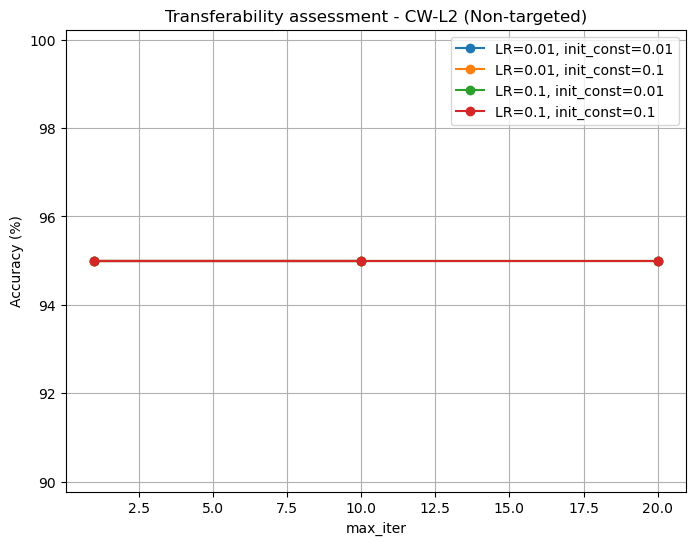
\includegraphics[width=0.6\textwidth]{images/cwtrasuntargl2.png}
            \caption{Accuracy vs max\_iter per Carlini \& Wagner $L2$ (Non-targeted)}
            \label{fig:cw_untarg_l2_acc}
        \end{figure}
        
        \begin{figure}[H]
            \centering
            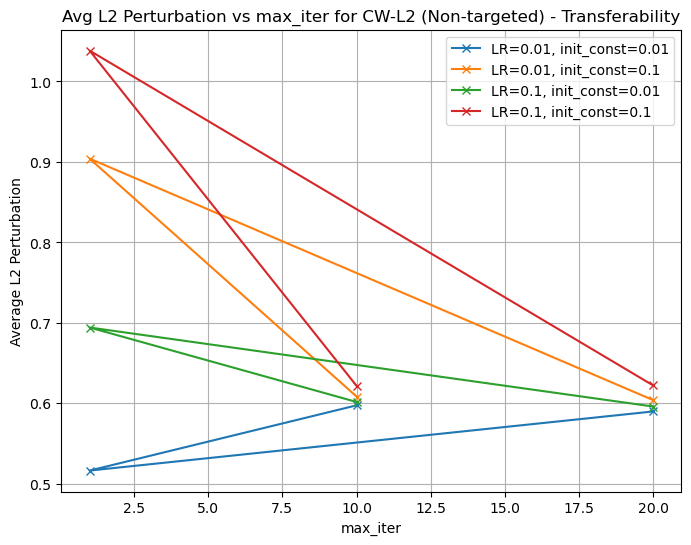
\includegraphics[width=0.6\textwidth]{images/cwtrasuntargl2-1.png}
            \caption{Avg $L^2$ Perturbation vs max\_iter per Carlini \& Wagner $L2$ (Non-targeted)}
            \label{fig:cw_untarg_l2_pert}
        \end{figure}
        
        \begin{figure}[H]
            \centering
            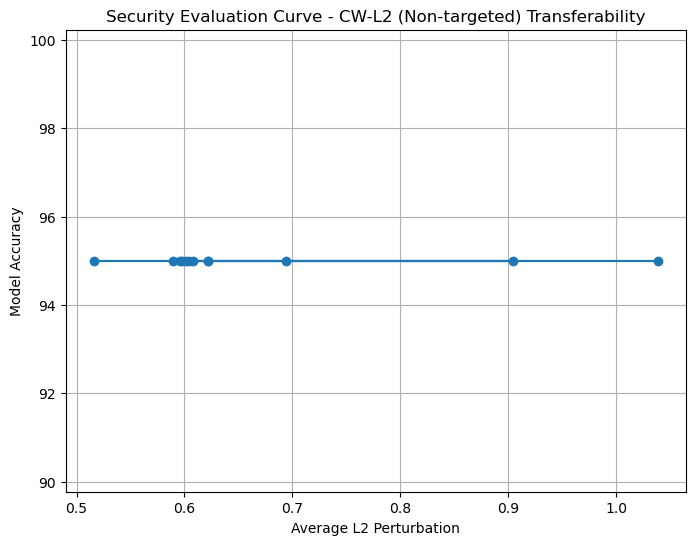
\includegraphics[width=0.6\textwidth]{images/cwtrasuntargl2sec.png}
            \caption{Security Evaluation Curve per Carlini \& Wagner $L2$ (Non-targeted)}
            \label{fig:cw_untarg_l2_sec}
        \end{figure}

        \subsection{Risultati}
            Nel contesto della valutazione di trasferibilità dell'attacco Carlini-Wagner in modalità non-targeted con norma L2, sono stati generati esempi avversari sulla rete sorgente NN1 e successivamente testati sulla rete target NN2. I risultati mostrano che l'attacco \textbf{non è riuscito a trasferirsi in alcuna configurazione}: in tutte le prove, l’accuratezza della rete target NN2 è rimasta invariata al $95\%$, ovvero identica al caso pulito.
            È interessante notare che, nonostante l'assenza di successo nella fase di trasferimento, le perturbazioni medie introdotte non erano trascurabili, con valori di norma $L2$ medi superiori a $0.5$ e massimi fino a $2.77$. Questo indica che il perturbatore ha effettivamente modificato l'immagine in modo misurabile, ma non in maniera sufficiente da compromettere le decisioni del classificatore target.
            Questo comportamento è coerente con quanto osservato in letteratura: gli attacchi Carlini-Wagner sono noti per essere ottimizzati in modo specifico per il modello su cui sono generati, e tendono a generare perturbazioni meno trasferibili rispetto ad altri attacchi come FGSM o BIM. La natura non lineare e altamente mirata dell’ottimizzazione, unita alla ricerca del minimo disturbo visibile, rende l’attacco meno generalizzabile ad architetture diverse.
            In Figura~\ref{fig:cwnt_transf_success},~\ref{fig:cwnt_transf_perturb},~\ref{fig:cwnt_transf_sec} si riportano rispettivamente:
            \begin{itemize}
                \item la curva di accuratezza su NN2 al variare di \texttt{max\_iter} e dei parametri dell’attacco;
                
                \item l’andamento della perturbazione media in norma L2 al crescere delle iterazioni;
                
                \item la Security Evaluation Curve che mostra l’assenza di compromissione anche in presenza di perturbazioni crescenti.
            \end{itemize}
            
            \begin{figure}[H]
                \centering
                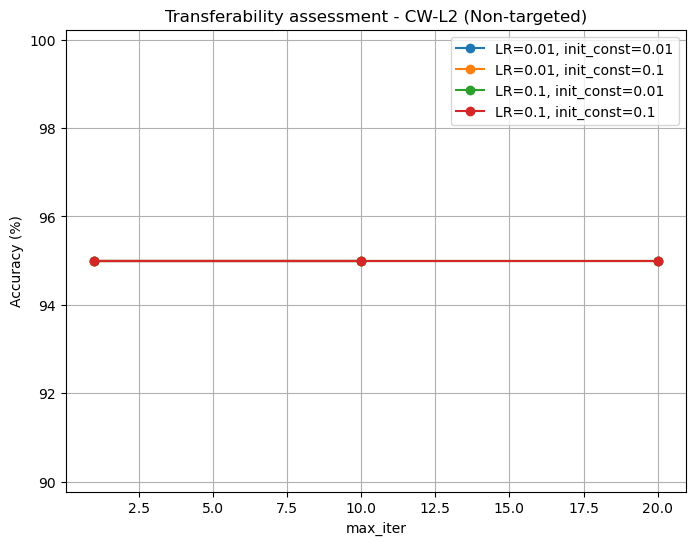
\includegraphics[width=0.55\textwidth]{images/cwtrasuntargl2.png}
                \caption{Transferability assessment - CW-$L2$ (Non-targeted)}
                \label{fig:cwnt_transf_success}
            \end{figure}
            
            \begin{figure}[H]
                \centering
                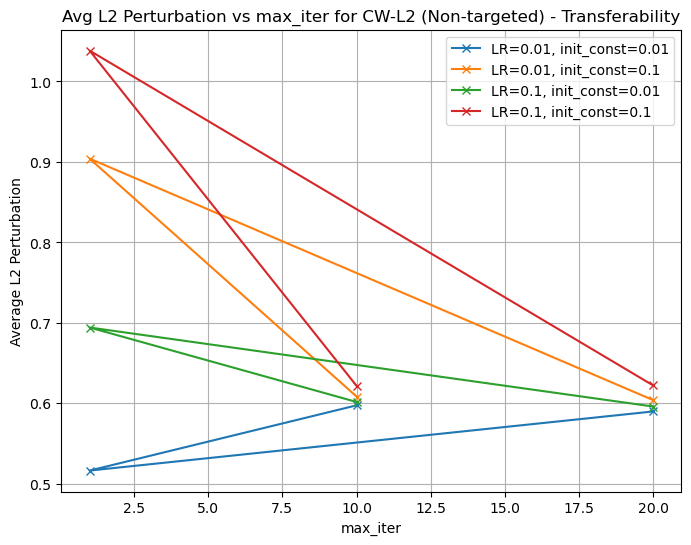
\includegraphics[width=0.55\textwidth]{images/cwtrasuntargl2-1.png}
                \caption{Average L2 Perturbation vs \texttt{max\_iter} - CW-L2 (Non-targeted)}
                \label{fig:cwnt_transf_perturb}
            \end{figure}
            
            \begin{figure}[H]
                \centering
                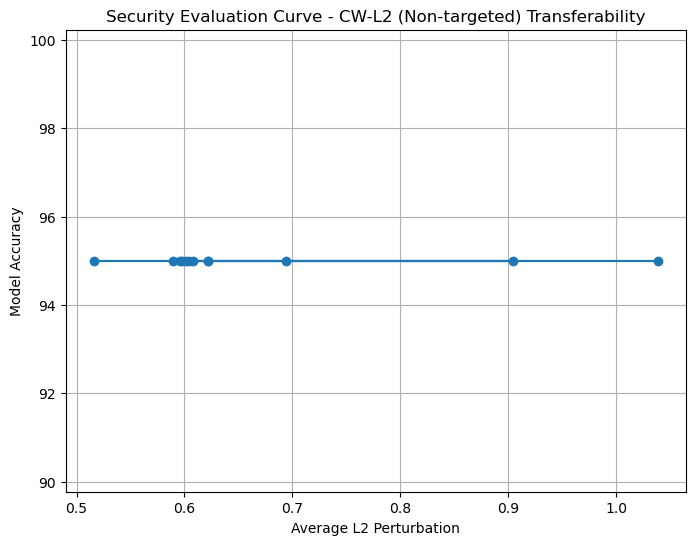
\includegraphics[width=0.55\textwidth]{images/cwtrasuntargl2sec.png}
                \caption{Security Evaluation Curve - CW-L2 (Non-targeted) Transferability}
                \label{fig:cwnt_transf_sec}
            \end{figure}
            
        \subsection{Analisi dei risultati}
            L’analisi complessiva dei risultati suggerisce che, pur essendo il Carlini-Wagner L2 un attacco efficace nel contesto white-box sul modello sorgente (NN1), \textbf{la sua capacità di trasferirsi ad altri modelli risulta estremamente limitata}. Tutte le configurazioni testate non sono riuscite ad alterare significativamente l’accuratezza del modello target (NN2), che è rimasta stabile al $95\%$.
            Questa evidenza conferma quanto riportato in letteratura, dove si sottolinea che gli attacchi CW, ottimizzati attraverso complesse funzioni obiettivo e vincoli di ottimalità su una specifica rete, \textbf{tendono a generare perturbazioni poco generalizzabili}. La mancanza di trasferibilità è particolarmente marcata nei casi in cui il modello target presenta architetture molto diverse rispetto a quello sorgente.
            Un ulteriore elemento di rilievo è che perturbazioni anche relativamente ampie in norma L2 non si sono tradotte in errori di classificazione su NN2. Ciò suggerisce che l’ottimizzazione avviene in una regione del manifold delle immagini molto legata alle specifiche caratteristiche apprese dal modello attaccato, rendendo il trasferimento meno probabile.
            In sintesi, i risultati ottenuti evidenziano come la potenza del Carlini-Wagner L2 sia fortemente legata al contesto white-box e pongono l’attenzione sulla necessità di combinare attacchi o progettare strategie più generalizzabili per analisi di robustezza cross-model.

    \section{Confronto tra gli Attacchi Non-Targeted}
        \begin{itemize}
          \item Gli attacchi iterativi come \textbf{BIM} e \textbf{PGD} ottengono i risultati più incisivi in termini di abbattimento dell’accuratezza su NN2, con valori inferiori al 42\%, a fronte di perturbazioni medie relativamente contenute ($\sim$0.06).
          
          \item L’attacco \textbf{FGSM}, pur essendo il più semplice, mostra un comportamento competitivo, ma richiede un livello di distorsione maggiore per ottenere un degrado simile.
          
          \item \textbf{DeepFool} si conferma altamente efficace in white-box, ma scarsamente trasferibile, con una perturbazione quasi nulla e una accuratezza residuale molto elevata su NN2 ($\sim$96\%).
          
          \item \textbf{Carlini-Wagner} mostra una trasferibilità significativa solo in presenza di learning rate elevati, risultando meno pericoloso in modalità black-box rispetto a PGD e BIM.
        \end{itemize}

        \noindent Nel complesso, gli attacchi iterativi proiettati (PGD e BIM) rappresentano la minaccia più rilevante in scenari black-box, grazie alla loro capacità di generare perturbazioni robuste e generalizzabili. Gli attacchi ottimizzati come CW sono invece più sensibili ai parametri e meno efficaci in trasferimento se non correttamente calibrati.

    \section{Trasferibilità dell'attacco FGSM Targeted}
        L'attacco \textbf{FGSM targeted}, applicato sulla rete NN1, è stato testato per verificarne la \textit{trasferibilità} verso il classificatore NN2 (basato su ResNet50). Lo scopo è determinare se le perturbazioni, progettate per forzare una classificazione errata verso una \textit{classe bersaglio} su NN1, riescano a generare lo stesso effetto anche su un modello con architettura differente.
        Il grafico in Figura~\ref{fig:fgsm_targeted_transfer} mostra l'andamento della \textit{Targeted Attack Success Rate} rispetto alla \textit{perturbazione media introdotta} nei campioni.

        \begin{figure}[H]
          \centering
          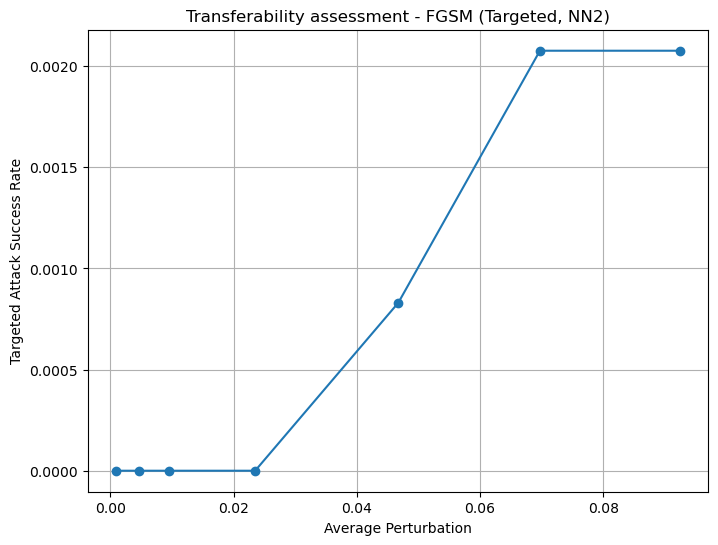
\includegraphics[width=0.65\textwidth]{images/fgsm_targeted_transferability.png}
          \caption{Transferability assessment - FGSM (Targeted, NN2).}
          \label{fig:fgsm_targeted_transfer}
        \end{figure}

        \subsection{Osservazioni}
            I risultati numerici indicano un tasso di successo nullo per valori di perturbazione media inferiori a $0.04$ e solo un modesto incremento nei casi più estremi:
                \begin{center}
                    \begin{tabular}{ccc}
                        \toprule
                        \textbf{Perturbazione media} & \textbf{L$_\infty$} & \textbf{Tasso di successo (\%)} \\
                        \midrule
                        0.0009 & 0.0010 & 0.00 \\
                        0.0047 & 0.0050 & 0.00 \\
                        0.0094 & 0.0100 & 0.00 \\
                        0.0235 & 0.0250 & 0.00 \\
                        0.0467 & 0.0500 & 0.08 \\
                        0.0697 & 0.0750 & 0.21 \\
                        0.0924 & 0.1000 & 0.21 \\
                        \bottomrule
                    \end{tabular}
                \end{center}

        \subsection{Analisi}
            L’attacco FGSM targeted si è dimostrato scarsamente trasferibile su NN2. Anche per livelli elevati di distorsione (L$\infty$ fino a 0.1), il tasso di successo rimane trascurabile (al massimo $\sim0.2\%$), a fronte di un successo superiore al 14\% osservato su NN1. Questo risultato conferma che l’attacco FGSM, basato su una singola iterazione lungo la direzione del gradiente, tende a produrre perturbazioni altamente specifiche per l’architettura bersaglio originale.
            In letteratura, è noto che gli attacchi \textit{targeted} sono generalmente meno trasferibili rispetto ai \textit{non-targeted}, a causa della maggiore precisione richiesta nel forzare la predizione verso una classe scelta dall’attaccante. Come evidenziato in studi come \textit{Liu et al., 2017} e \textit{Goodfellow et al., 2015}, la trasferibilità tende a decrescere all’aumentare della specificità dell’obiettivo dell’attacco.

    \section{Trasferibilità dell'attacco BIM Targeted}
        In questo esperimento è stata analizzata la trasferibilità dell’attacco \textbf{Basic Iterative Method (BIM)}, in modalità \textit{targeted}, verso il classificatore NN2 (ResNet50). L’obiettivo è valutare se le perturbazioni costruite per forzare la predizione di NN1 verso una specifica classe siano efficaci anche su una rete architetturalmente distinta.
        Il grafico in Figura~\ref{fig:bim_targeted_transfer} rappresenta l’evoluzione del \textit{Targeted Attack Success Rate} in funzione della \textit{perturbazione media}, variando i parametri \texttt{max\_iter} e $\epsilon$.

        \begin{figure}[H]s
          \centering
          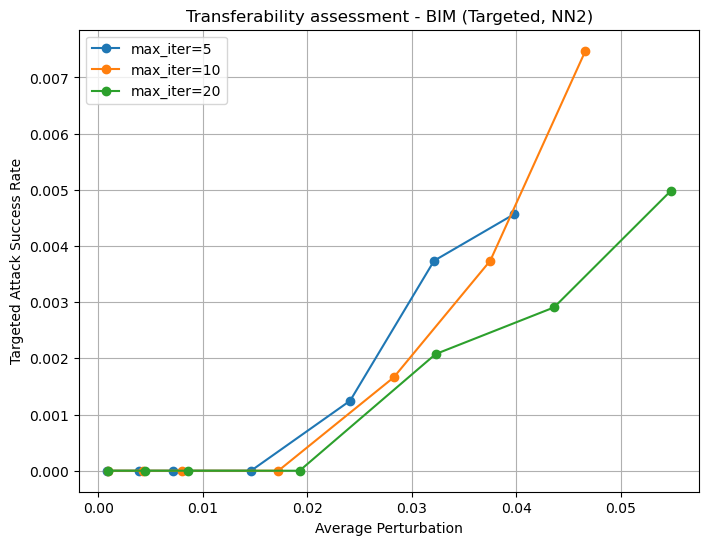
\includegraphics[width=0.7\textwidth]{images/bim_targeted_transferability.png}
          \caption{Transferability assessment - BIM (Targeted, NN2).}
          \label{fig:bim_targeted_transfer}
        \end{figure}

        \subsection{Risultati}
            I risultati mostrano che l'attacco BIM targeted mantiene una scarsa capacità di trasferirsi a NN2. Per perturbazioni deboli (L$\infty \leq 0.025$), il tasso di successo è nullo indipendentemente dal numero di iterazioni. Solo a partire da $\epsilon = 0.05$, si osserva un leggero incremento:
            
            \begin{itemize}
              \item Per $\epsilon = 0.05$, \texttt{max\_iter} = 5, il tasso di successo è pari allo 0.12\%.
              \item Aumentando a \texttt{max\_iter} = 10 e 20, si ottengono rispettivamente successi dello 0.17\% e 0.21\%.
              \item Con $\epsilon = 0.1$, si raggiungono i valori massimi osservati: fino allo 0.75\% con \texttt{max\_iter} = 10.
            \end{itemize}

            \noindent Nonostante la maggiore potenza dell’attacco iterativo rispetto al FGSM, i risultati confermano che la \textbf{trasferibilità degli attacchi targeted è intrinsecamente limitata}, in particolare quando si considerano modelli profondamente diversi (NN1 vs NN2).

        \subsection{Discussione}
            BIM, essendo una versione iterativa di FGSM, produce perturbazioni localmente più efficaci nel dominio del modello bersaglio. Tuttavia, queste perturbazioni sembrano ottimizzate in modo troppo specifico per l’architettura NN1 e raramente riescono a guidare NN2 verso la classe bersaglio desiderata.
            Come evidenziato in letteratura (\textit{Liu et al., 2017}), gli attacchi \textit{targeted} richiedono una precisa manipolazione della distribuzione delle attivazioni intermedie, il che riduce la probabilità di successo su modelli non identici. Inoltre, la strategia di trasferire classi bersaglio tramite mappatura ciclica potrebbe accentuare questa difficoltà.

    \section{Trasferibilità dell'attacco PGD Targeted}
        L’attacco \textbf{Projected Gradient Descent (PGD)} consente di esplorare con maggiore efficacia il dominio locale di input, massimizzando la probabilità di ingannare il classificatore. In questa sezione ne analizziamo la trasferibilità, in modalità \textit{targeted}, dalla rete NN1 alla rete ResNet50 (NN2).
        Il grafico di Figura~\ref{fig:pgd_targeted_transfer} mostra il tasso di successo dell’attacco in funzione della perturbazione media, al variare del parametro \texttt{max\_iter}.
        
        \begin{figure}[H]
          \centering
          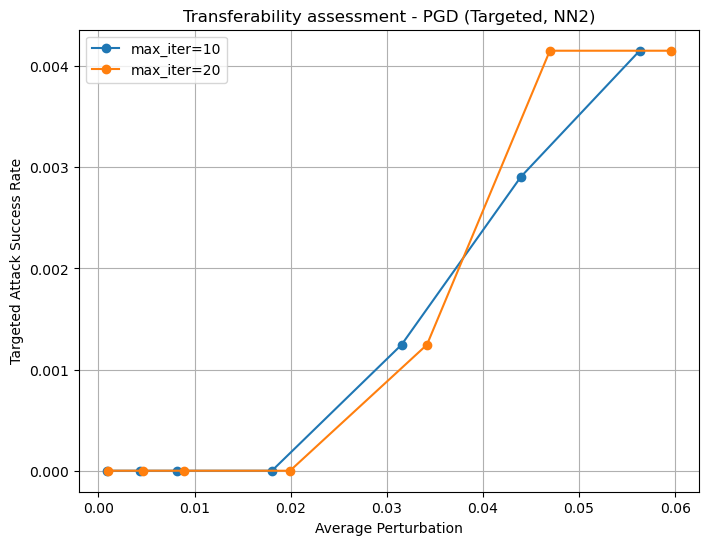
\includegraphics[width=0.7\textwidth]{images/pgd_targeted_transferability.png}
          \caption{Transferability assessment - PGD (Targeted, NN2).}
          \label{fig:pgd_targeted_transfer}
        \end{figure}

        \subsection{Risultati}
            I risultati indicano che la probabilità di successo dell’attacco PGD targeted su NN2 è estremamente bassa. Nella maggior parte dei casi, il tasso di successo rimane nullo fino a perturbazioni superiori a 0.03. Alcune osservazioni chiave includono:
            
            \begin{itemize}
              \item Per $\epsilon \leq 0.025$, il \textit{Targeted Success Rate} è sempre 0\%.
              \item A partire da $\epsilon = 0.05$, si ottiene un successo marginale dello 0.12\%.
              \item Con $\epsilon = 0.075$ e \texttt{max\_iter} = 20, il successo sale fino allo 0.42\%.
              \item Aumentare ulteriormente \texttt{max\_iter} non produce miglioramenti significativi oltre tale soglia.
            \end{itemize}
            
        \subsection{Discussione}
            Sebbene PGD sia riconosciuto in letteratura (\textit{Madry et al., 2018}) come uno degli attacchi più robusti in scenari \textit{white-box}, i risultati ottenuti suggeriscono che in modalità \textit{targeted} esso non riesca a trasferirsi efficacemente a modelli differenti.
            Il motivo risiede nella natura \textit{direzionale} dell’attacco. PGD, infatti, cerca specificamente di forzare il modello a classificare l'immagine come una classe target, ottimizzando una traiettoria molto precisa nello spazio delle immagini. Questa traiettoria, sebbene efficace su NN1, perde coerenza semantica quando valutata su NN2.
            Anche la componente stocastica del PGD (un solo \texttt{random\_init} in questo caso) potrebbe non essere sufficiente a generare perturbazioni generalizzabili ad altri modelli. Un incremento del numero di inizializzazioni casuali potrebbe migliorare leggermente la trasferibilità, ma a scapito del tempo computazionale.

        \subsection{Conclusione}
            La trasferibilità del PGD targeted su NN2 risulta limitata. Anche con perturbazioni consistenti ($\epsilon = 0.1$), il tasso di successo non supera lo 0.42\%. Questo comportamento conferma quanto osservato per gli altri attacchi targeted, l’ottimizzazione verso una classe specifica tende a produrre perturbazioni fortemente legate alla rete su cui vengono generate, rendendo difficile la generalizzazione cross-architettura.

    \section{Trasferibilità dell'attacco Targeted Carlini-Wagner L$\infty$ }
        L'attacco \textit{Carlini-Wagner} con norma L$\infty$ è stato eseguito in modalità \textit{targeted} sulla rete NN1 e successivamente è stata valutata la sua trasferibilità su NN2. L’obiettivo era verificare se gli esempi avversari potessero forzare NN2 a classificare le immagini secondo le etichette target predefinite, ossia la classe successiva modulo $N$.

        \subsection{Parametri dell'esperimento}
            L'attacco è stato testato su un sottoinsieme di 20 immagini del test set, selezionate casualmente.
            I parametri esplorati includono:
                \begin{itemize}
                  \item \textbf{Learning rate}: \texttt{0.01}, \texttt{0.1}
                  \item \textbf{Max iterazioni}: \texttt{1}, \texttt{10}, \texttt{20}
                  \item \textbf{Initial constant}: \texttt{0.01}, \texttt{0.1}
                \end{itemize}

        \subsection{Risultati}
            I risultati mostrano che, nonostante la variazione dei parametri, \textbf{il tasso di successo dell'attacco targeted trasferito è rimasto costantemente pari a 0\%} per tutte le combinazioni. Questo indica che nessun esempio avversario ha indotto NN2 a classificare correttamente secondo la classe target desiderata.
            In particolare, anche nei casi in cui la perturbazione media era relativamente elevata (ad esempio con \texttt{LR=0.1}, \texttt{max\_iter=1}), la rete NN2 ha sempre fallito nel classificare le immagini nella classe target. Le curve riportate confermano questi risultati:
                \begin{itemize}
                  \item \textbf{Figura \ref{fig:cwlinf-transfer-accuracy}} mostra il \textit{Targeted Success Rate} rispetto a \texttt{max\_iter}, evidenziando valori nulli indipendentemente dai parametri.
                  
                  \item \textbf{Figura \ref{fig:cwlinf-transfer-perturb}} rappresenta la perturbazione media introdotta in funzione di \texttt{max\_iter}. Si osservano picchi iniziali che si annullano completamente per iterazioni più elevate.
                  
                  \item \textbf{Figura \ref{fig:cwlinf-transfer-sec}} è la \textit{Security Evaluation Curve}, che evidenzia come l'incremento della perturbazione non si traduca in alcun successo dell’attacco.
                \end{itemize}
            
            \begin{figure}[H]
              \centering
              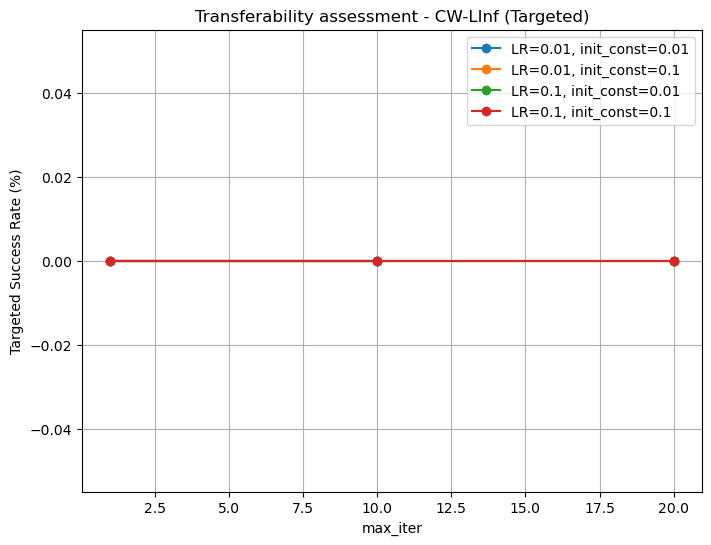
\includegraphics[width=0.65\textwidth]{images/cwlinf_transfer_accuracy.png}
              \caption{Transferability assessment - CW-L$\infty$ (Targeted)}
              \label{fig:cwlinf-transfer-accuracy}
            \end{figure}
            
            \begin{figure}[H]
              \centering
              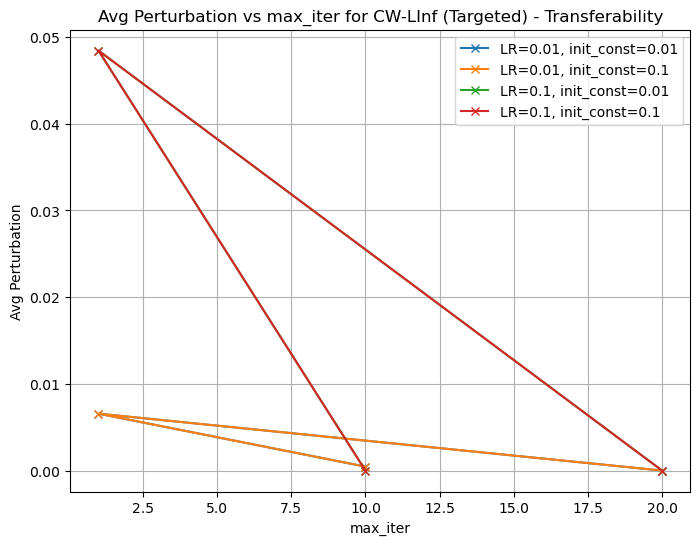
\includegraphics[width=0.65\textwidth]{images/cwlinf_transfer_perturb.png}
              \caption{Avg Perturbation vs max\_iter - CW-L$\infty$ (Targeted) - Transferability}
              \label{fig:cwlinf-transfer-perturb}
            \end{figure}
            
            \begin{figure}[H]
              \centering
              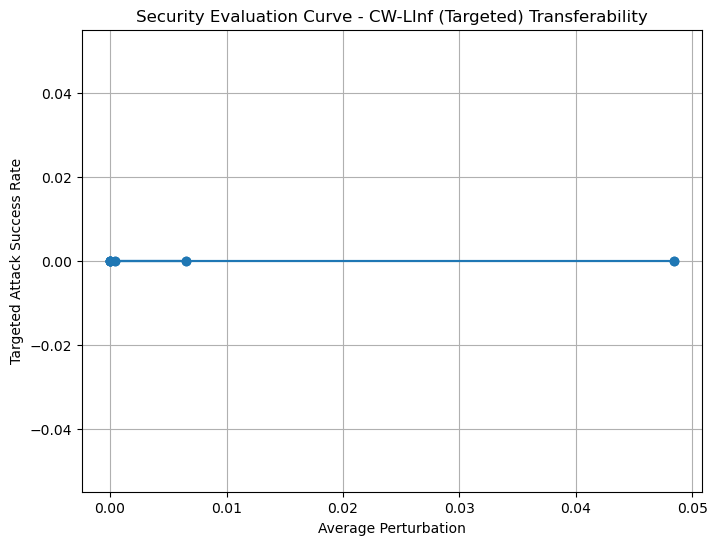
\includegraphics[width=0.65\textwidth]{images/cwlinf_transfer_sec_eval.png}
              \caption{Security Evaluation Curve - CW-L$\infty$ (Targeted) - Transferability}
              \label{fig:cwlinf-transfer-sec}
            \end{figure}

        \subsection{Discussione}
            Il comportamento osservato è coerente con quanto riportato in letteratura: gli attacchi Carlini-Wagner, pur essendo potenti sul modello sorgente, tendono a non trasferirsi efficacemente. Questo accade perché il metodo CW ottimizza perturbazioni molto specifiche rispetto alla funzione obiettivo e ai gradienti del modello attaccato, producendo perturbazioni difficili da generalizzare su modelli con architettura diversa.
            Inoltre, nella modalità targeted, la condizione è ancora più restrittiva, in quanto non è sufficiente ingannare il classificatore, ma bisogna forzarlo a produrre una specifica predizione. Ciò rende la trasferibilità ancora meno probabile.

    \section{Trasferibilità dell'attacco Targeted Carlini-Wagner L2}
        In questa sezione analizziamo la capacità di trasferimento verso NN2 degli adversarial samples generati tramite l’attacco \textbf{Carlini \& Wagner con norma L2} in modalità \textit{targeted}. A differenza della versione \textit{error-generic}, l’obiettivo di questo attacco è forzare il classificatore ad assegnare un’etichetta specifica (target) a ciascuna immagine, rendendo l’analisi della trasferibilità particolarmente interessante in un contesto black-box.
        I risultati sono riportati nei seguenti grafici.
        
        \begin{figure}[H]
          \centering
          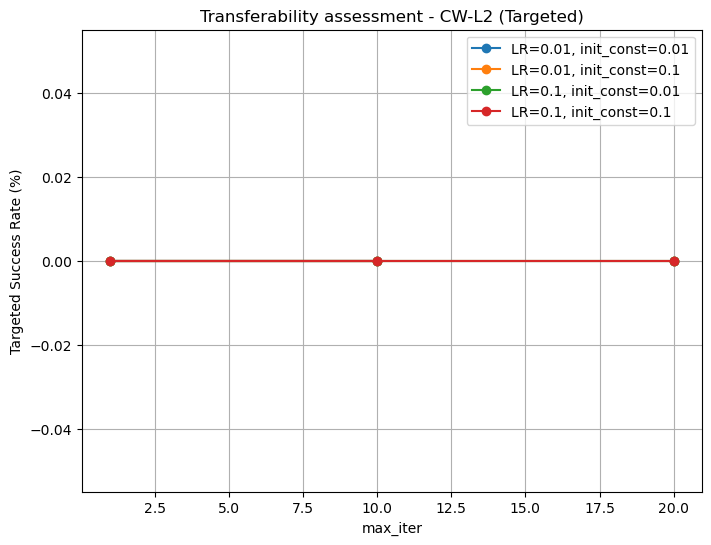
\includegraphics[width=0.75\textwidth]{images/cwtrastargl2.png}
          \caption{Transferability assessment - CW-L2 (Targeted)}
        \end{figure}
        
        \begin{figure}[H]
          \centering
          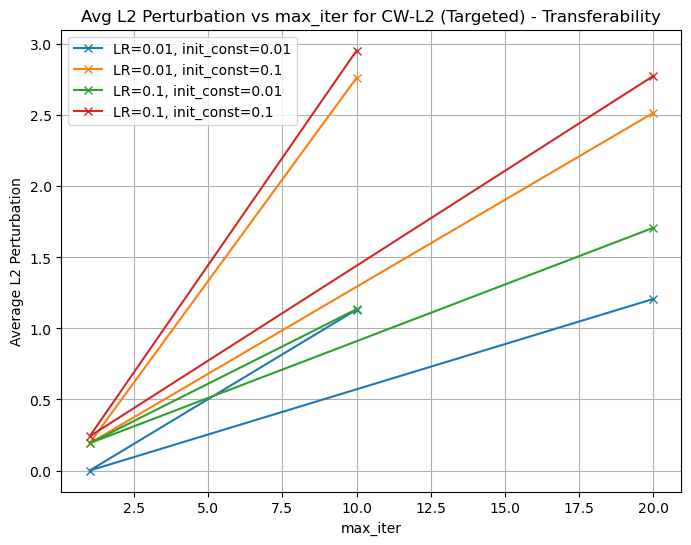
\includegraphics[width=0.75\textwidth]{images/cwtrastargl2-1.png}
          \caption{Avg L2 Perturbation vs max\_iter for CW-L2 (Targeted) - Transferability}
        \end{figure}
        
        \begin{figure}[H]
          \centering
          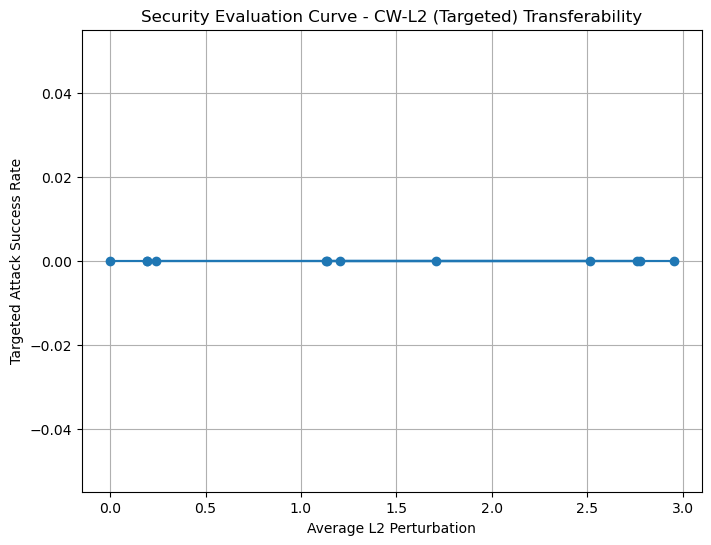
\includegraphics[width=0.75\textwidth]{images/cwtrastargl2sec.png}
          \caption{Security Evaluation Curve - CW-L2 (Targeted) Transferability}
        \end{figure}

        \subsection{Analisi dei risultati}
            Come evidenziato dai grafici, nonostante la presenza di perturbazioni anche significative (con valori medi di norma L2 superiori a 2.5 per alcune configurazioni), la \textbf{success rate} dell’attacco su NN2 è risultata nulla in tutti i casi analizzati. Nemmeno per valori elevati di \texttt{initial\_const} e \texttt{max\_iter} è stato ottenuto un singolo successo nell’indurre NN2 a classificare l’immagine nella classe target desiderata.
            Questo risultato conferma la scarsa trasferibilità degli attacchi Carlini-Wagner L2 in modalità targeted, già osservata in letteratura. Tali attacchi tendono infatti a produrre perturbazioni molto precise e specifiche per l'architettura, difficilmente generalizzabili a modelli differenti, specialmente quando la struttura (NN1 vs NN2) cambia significativamente.
            L’andamento della curva di sicurezza mostra inoltre una decisa separazione tra l’aumento della perturbazione e il mancato guadagno in termini di successo, suggerendo un’inefficacia strutturale nella generalizzazione dell’attacco.

    \section{Confronto sulla Trasferibilità degli Attacchi Targeted}
        Come già detto in precedenza, la misura utilizzata per quantificare l'efficacia del trasferimento è la \textit{Targeted Attack Success Rate}, ovvero la percentuale di campioni per cui la rete target ha predetto correttamente la classe obiettivo imposta dall'attacco.
        I risultati confermano un comportamento coerente con quanto noto in letteratura:
            \begin{itemize}
                \item \textbf{FGSM}: presenta un successo di trasferibilità molto basso (max $\approx 0.21\%$), anche per valori elevati di perturbazione. Questo è coerente con la sua natura one-step e la direzionalità debole della perturbazione.
                
                \item \textbf{BIM} e \textbf{PGD}: migliorano leggermente rispetto a FGSM (fino a circa $0.75\%$), ma restano comunque scarsamente efficaci in ottica targeted transfer. Entrambi sono gradient-based iterativi, ma risultano sensibili alla specificità del modello.
                
                \item \textbf{CW (L$\infty$ e L$2$)}: completamente inefficace nella modalità targeted. Nessuna configurazione di iperparametri ha portato a un singolo caso di successo, a testimonianza della forte specializzazione dell'attacco.
            \end{itemize}

        \noindent Riassumendo, tutti gli attacchi targeted presentano \textbf{trasferibilità estremamente limitata}, con tassi di successo spesso inferiori all’1\%. Questo comportamento è dovuto al fatto che le perturbazioni targeted tendono ad essere molto precise e \textit{model-specific}, ottimizzate per portare la rete ad una classe ben definita, e quindi scarsamente generalizzabili su modelli differenti.
    \chapter{Detection of Adversarial Samples}
    \section{Misure di Difesa: Rilevamento di \textit{Adversarial Samples}}
        Per contrastare il fenomeno degli \textit{adversarial samples}, una strategia efficace consiste nell’introduzione di un \textbf{rilevatore di adversarial samples} a monte del sistema di classificazione. In particolare, in questo lavoro è stato adottato un \textit{Binary Input Detector} (BID), una rete neurale binaria il cui compito è discriminare tra input \textit{benigni} (ovvero non manipolati) e input \textit{adversarial}.
        L’approccio adottato si basa sull’assunzione che gli adversarial examples, pur essendo visivamente simili agli originali, presentino caratteristiche distribuzionali diverse nello spazio delle rappresentazioni apprese dal modello. Queste differenze possono essere apprese da un classificatore binario, opportunamente addestrato su un dataset contenente sia immagini originali sia immagini avversarie generate con i diversi attacchi eseguiti in precedenza.
        Il detector utilizzato è stato pre-addestrato su immagini preprocessate a bassa risoluzione ($32\times32$ pixel), con una architettura compatibile con \texttt{TensorFlowV2Classifier} della libreria \texttt{ART}. La scelta di un modello leggero e binario consente una facile integrazione nella pipeline del sistema di riconoscimento, con un buon compromesso tra accuratezza, velocità e capacità di generalizzazione.

    \section{Adversarial Detection come difesa proattiva}
        Il rilevamento di input avversari è una delle strategie difensive più studiate nel campo della sicurezza dei sistemi di machine learning. A differenza delle tecniche di robust training, che cercano di rendere il modello principale intrinsecamente più resistente agli attacchi, i meccanismi di \textit{detection} agiscono come un filtro a monte del classificatore, con l’obiettivo di intercettare e bloccare campioni sospetti prima che possano compromettere il processo decisionale.
        Questa impostazione si inserisce nel più ampio contesto delle \textbf{difese proattive}, in cui l’input viene valutato separatamente rispetto alla rete target. In particolare, i \textit{Binary Input Detectors} (BID) rappresentano un approccio semplice ma efficace: un classificatore binario viene addestrato su un dataset contenente sia immagini originali che malevole, con l’obiettivo di imparare a distinguere le due distribuzioni.
        L’assunzione di fondo è che, anche se le perturbazioni sono impercettibili a livello visivo, esse modificano in modo sistematico le rappresentazioni interne apprese dal modello, generando anomalie statistiche sfruttabili dal rilevatore. Tuttavia, questa strategia non è priva di limiti, infatti un BID è fortemente dipendente dal tipo di attacchi osservati durante l’addestramento e può risultare meno efficace contro tecniche mai viste o particolarmente sofisticate. Inoltre, come evidenziato in letteratura, alcuni detector possono essere facilmente ingannati da attacchi \textit{transfer-based} oppure \textit{adaptive}, in cui l’attaccante è a conoscenza della presenza del detector e ne ottimizza la perdita in fase di generazione dell’attacco.
        Un ulteriore elemento critico riguarda la \textit{generalizzazione}, poichè il rilevatore potrebbe imparare a riconoscere pattern specifici di un attacco piuttosto che le proprietà generali degli adversarial samples. Ciò può portare a overfitting e a una drastica riduzione dell’efficacia su dataset reali o su attacchi fuori distribuzione.
        Nel contesto di questo progetto, l’uso di un BID pre-addestrato su immagini preprocessate a bassa risoluzione consente di valutare in modo controllato la capacità del detector di distinguere tra classi avversarie e legittime. Nonostante le limitazioni insite in questo approccio, i risultati ottenuti mostrano che, almeno nel dominio considerato e con attacchi di intensità moderata, la strategia di detection risulta efficace e rappresenta una valida prima linea di difesa contro input manipolati.
        Nel seguito, vengono descritte le procedure di preprocessing, addestramento e validazione del rilevatore, accompagnate da un'analisi quantitativa delle performance ottenute.

    \section{Implementazione del Detector}
        L’intero processo di implementazione del detector di adversarial samples, si articola in tre fasi principali: preprocessing dei dati, addestramento del modello e valutazione su un insieme di validazione.
        
        \subsection{Preprocessing e Costruzione del Dataset}
            I dati utilizzati per l’addestramento e la validazione del detector sono stati ottenuti a partire dal test set originale, composto da immagini \textit{benigne} di volti provenienti dal dataset VGGFace2. Le immagini, inizialmente nel formato $160\times160\times3$, sono state ridimensionate a $32\times32\times3$ per renderle compatibili con l’input richiesto dal modello di rilevamento.
            In parallelo, sono stati riutilizzati i campioni \textit{adversarial} generati mediante l’utilizzo dei sei attacchi eseguiti in precedenza: FGSM, BIM, PGD error-generic e le rispettive versioni \textit{targeted}. Per evitare problemi di bias, sono stati esclusi gli attacchi DeepFool e Carlini-Wagner, i quali non coprono l’intero test set.
            Per ciascun attacco, le immagini avversarie sono state preprocessate con la stessa procedura delle immagini originali. \\
            Il dataset finale per l’addestramento del detector è stato costruito unendo:
                \begin{itemize}
                    \item Immagini \textbf{benigne} con etichetta 0,
                    \item Immagini \textbf{adversarial} con etichetta 1.
                \end{itemize}
    
            \noindent La divisione tra training e validation set è stata effettuata mediante \texttt{train\_test\_split}, mantenendo la proporzione 80\% / 20\% . Al termine, i dati sono stati \texttt{mescolati} per evitare correlazioni tra ordine e label e quindi   ottenere maggior randomicità.
    
        \subsection{Addestramento del Detector}
            Il rilevatore è stato implementato tramite il wrapper \texttt{BinaryInputDetector} fornito dalla libreria ART. Al suo interno è impiegato un classificatore binario costruito come oggetto \texttt{TensorFlowV2Classifier}, caricato da un modello pre-addestrato salvato nel file \texttt{BID\_eps=0.05.h5}.
            L’addestramento è stato effettuato sul dataset binario costruito in precedenza, utilizzando una funzione di perdita binaria cross-entropy e l’ottimizzatore Adam con tasso di apprendimento 0.001. Sono state effettuate 10 epoche di training con batch size pari a 64.
    
        \subsection{Valutazione sul Validation Set}
            Il rilevatore è stato testato su un validation set costituito da 3374 immagini, di cui 482 appartenenti alla classe \textit{benign} e 2892 alla classe \textit{adversarial}, ottenute dagli attacchi citati in precedenza. I risultati della classificazione binaria sono sintetizzati nella matrice di confusione riportata in Figura~\ref{fig:conf_matrix}.
            Dall’analisi dei dati emerge un comportamento particolarmente conservativo da parte del modello: tutti i campioni benigni sono stati classificati correttamente, senza generare alcun falso positivo. Questo risultato è di particolare interesse per l’affidabilità di un sistema reale, poiché evita che input legittimi vengano bloccati erroneamente dal sistema di difesa. Tuttavia, circa il 24\% dei campioni adversarial (684 su 2892) non è stato rilevato, venendo etichettato erroneamente come benigno. Questo porta a un richiamo (\textit{recall}) per la classe adversarial pari al 76.36\%, mentre la precisione rimane perfetta (1.00), poiché tutti i campioni rilevati come falsi lo erano realmente.
            Complessivamente, il sistema raggiunge un’accuratezza dell’79.73\%, con un F1-score di 0.87 per la classe adversarial e 0.58 per la classe benign. Quest’ultima differenza riflette uno sbilanciamento nella strategia decisionale del modello, che tende a favorire la sicurezza rispetto all’usabilità: rileva con estrema cautela gli attacchi, evitando qualsiasi classificazione errata di input benigni, ma accetta il compromesso di non intercettare la totalità dei campioni avversari.
            L’immagine in Figura~\ref{fig:conf_matrix} illustra bene questo comportamento. I valori lungo la diagonale confermano la capacità del modello di apprendere le caratteristiche principali dei dati, mentre la presenza significativa di falsi negativi (684) nella parte inferiore sinistra evidenzia il margine di miglioramento nella generalizzazione su esempi avversari più sofisticati o meno evidenti.
            Nel complesso, i risultati ottenuti indicano che il rilevatore è in grado di operare in modo affidabile in contesti in cui è cruciale minimizzare i falsi allarmi. Tuttavia, per aumentare ulteriormente la robustezza, potrebbe essere utile integrare strategie complementari, come tecniche di data augmentation.
    
        \begin{figure}[H]
            \centering
            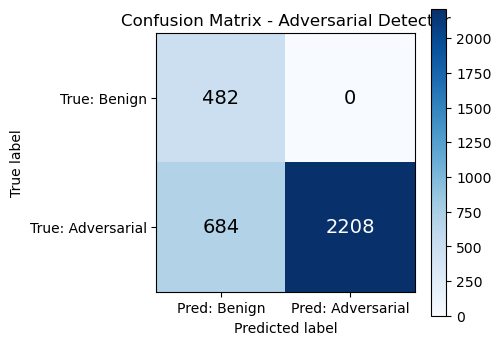
\includegraphics[width=0.6\textwidth]{images/confusionMatrix.png}
            \caption{Matrice di confusione del detector sul validation set.}
            \label{fig:conf_matrix}
        \end{figure}
    \chapter{Considerazioni finali e sviluppi futuri}
    Lo studio condotto ha permesso di valutare la robustezza di un sistema di riconoscimento facciale pre-addestrato rispetto a diversi attacchi avversari e di testare una tecnica difensiva per mitigarne gli effetti. I risultati ottenuti confermano l’efficacia delle perturbazioni generate con metodi noti e mostrano come anche modifiche impercettibili all’occhio umano possano compromettere drasticamente le prestazioni del modello.
    Tuttavia, il lavoro è stato svolto all’interno di un contesto con risorse limitate, sia in termini di tempo computazionale che di disponibilità hardware. Questo ha imposto alcune scelte progettuali conservative, come la generazione di un numero contenuto di esempi avversari e un numero limitato di iterazioni per gli attacchi più onerosi, come \textit{Carlini Wagner} o \textit{DeepFool}. \\
    In un contesto ideale, privo di tali vincoli e con l’accesso a maggiori risorse computazionali (ad esempio più GPU e memoria disponibile), sarebbe possibile estendere l’esperimento a un’analisi più approfondita e sistematica.
    In particolare, si potrebbero aumentare sensibilmente il numero di campioni avversari generati e le iterazioni degli algoritmi di attacco, migliorando così l’analisi quantitativa e qualitativa degli effetti prodotti sul classificatore.
    Un altro aspetto critico emerso riguarda il \textbf{meccanismo di rilevamento degli adversarial examples}: sebbene esso non produca falsi positivi, si è osservata una significativa percentuale di \textit{falsi negativi}, ovvero campioni avversari che non vengono riconosciuti come tali. Questo comportamento limita l’affidabilità complessiva del sistema. Un possibile sviluppo futuro potrebbe quindi riguardare l’ottimizzazione del detector, integrando tecniche più avanzate come analisi delle attivazioni interne, classificatori addestrati ad hoc o approcci basati su \textit{ensemble}.

\end{document}